\documentclass[11pt,letterpaper,oneside]{report}

\usepackage[utf8]{inputenc}
\usepackage[T1]{fontenc}
\usepackage[provide=*,spanish]{babel}
\usepackage{lmodern}
\usepackage[top=2.25cm,bottom=2.35cm,left=2.45cm,right=2.35cm]{geometry}
\usepackage{xcolor}
\usepackage{graphicx}
\usepackage{booktabs}
\usepackage{tabularx}
\usepackage{longtable}
\usepackage{array}
\usepackage{amsmath}
\usepackage{amssymb}
\usepackage{float}
\usepackage{hyperref}

\definecolor{navy}{HTML}{071126}
\definecolor{blue}{HTML}{2563EB}
\definecolor{cyan}{HTML}{0891B2}
\definecolor{violet}{HTML}{7C3AED}
\definecolor{green}{HTML}{15803D}
\definecolor{red}{HTML}{B42318}
\definecolor{orange}{HTML}{C2410C}
\definecolor{soft}{HTML}{F1F5F9}
\definecolor{codebg}{HTML}{F7F9FC}
\definecolor{codeborder}{HTML}{CBD5E1}
\definecolor{darkgray}{HTML}{334155}

\hypersetup{
  colorlinks=true,
  linkcolor=blue,
  urlcolor=cyan,
  citecolor=violet,
  pdftitle={Compiscript Semantic IDE -- Informe técnico ampliado del Proyecto 1},
  pdfauthor={DragonsSlayers 2.0},
  pdfsubject={Análisis léxico, sintáctico y semántico, tabla de símbolos e IDE},
  pdfkeywords={Compiscript, ANTLR, TypeScript, análisis semántico, tabla de símbolos}
}

\pagestyle{plain}

\setlength{\parindent}{0pt}
\setlength{\parskip}{0.62em}
\setlength{\emergencystretch}{3em}
\renewcommand{\arraystretch}{1.18}
\setcounter{secnumdepth}{3}
\setcounter{tocdepth}{2}
\raggedbottom

\newcolumntype{Y}{>{\raggedright\arraybackslash}X}
\newcolumntype{C}{>{\centering\arraybackslash}X}
% \path permite cortes de línea seguros en rutas largas dentro de tablas.
\newcommand{\archivo}[1]{\path{#1}}
\newcommand{\codigo}[1]{\texttt{#1}}
\newcommand{\estado}[1]{\textcolor{green}{\textbf{#1}}}
\newcommand{\fase}[1]{\textcolor{blue}{\textbf{#1}}}
\newcommand{\diag}[1]{\textcolor{red}{\texttt{#1}}}
\newcommand{\Compiscript}{\textsc{Compiscript}}
\newcommand{\ANTLR}{ANTLR 4}

\newenvironment{resumenclave}
  {\begin{center}\begin{minipage}{0.93\textwidth}\color{darkgray}
   \hrule\vspace{0.55em}\textbf{Idea clave.}\ }
  {\vspace{0.55em}\hrule\end{minipage}\end{center}}

\begin{document}
\hypersetup{pageanchor=false}

\begin{titlepage}
  \pagecolor{navy}
  \color{white}
  \centering
  \vspace*{0.9cm}
  {\Large Universidad del Valle de Guatemala\par}
  \vspace{0.25cm}
  {\large Facultad de Ingeniería\par}
  {\large Construcción de Compiladores -- CC-3032, sección 10\par}
  \vfill
  {\Huge\bfseries Compiscript Semantic IDE\par}
  \vspace{0.4cm}
  {\LARGE Proyecto 1\par}
  \vspace{0.25cm}
  {\Large Análisis semántico, tabla de símbolos e IDE\par}
  \vspace{0.7cm}
  \IfFileExists{../../presentation/assets/compiler-pipeline-neobrutalist.png}{
    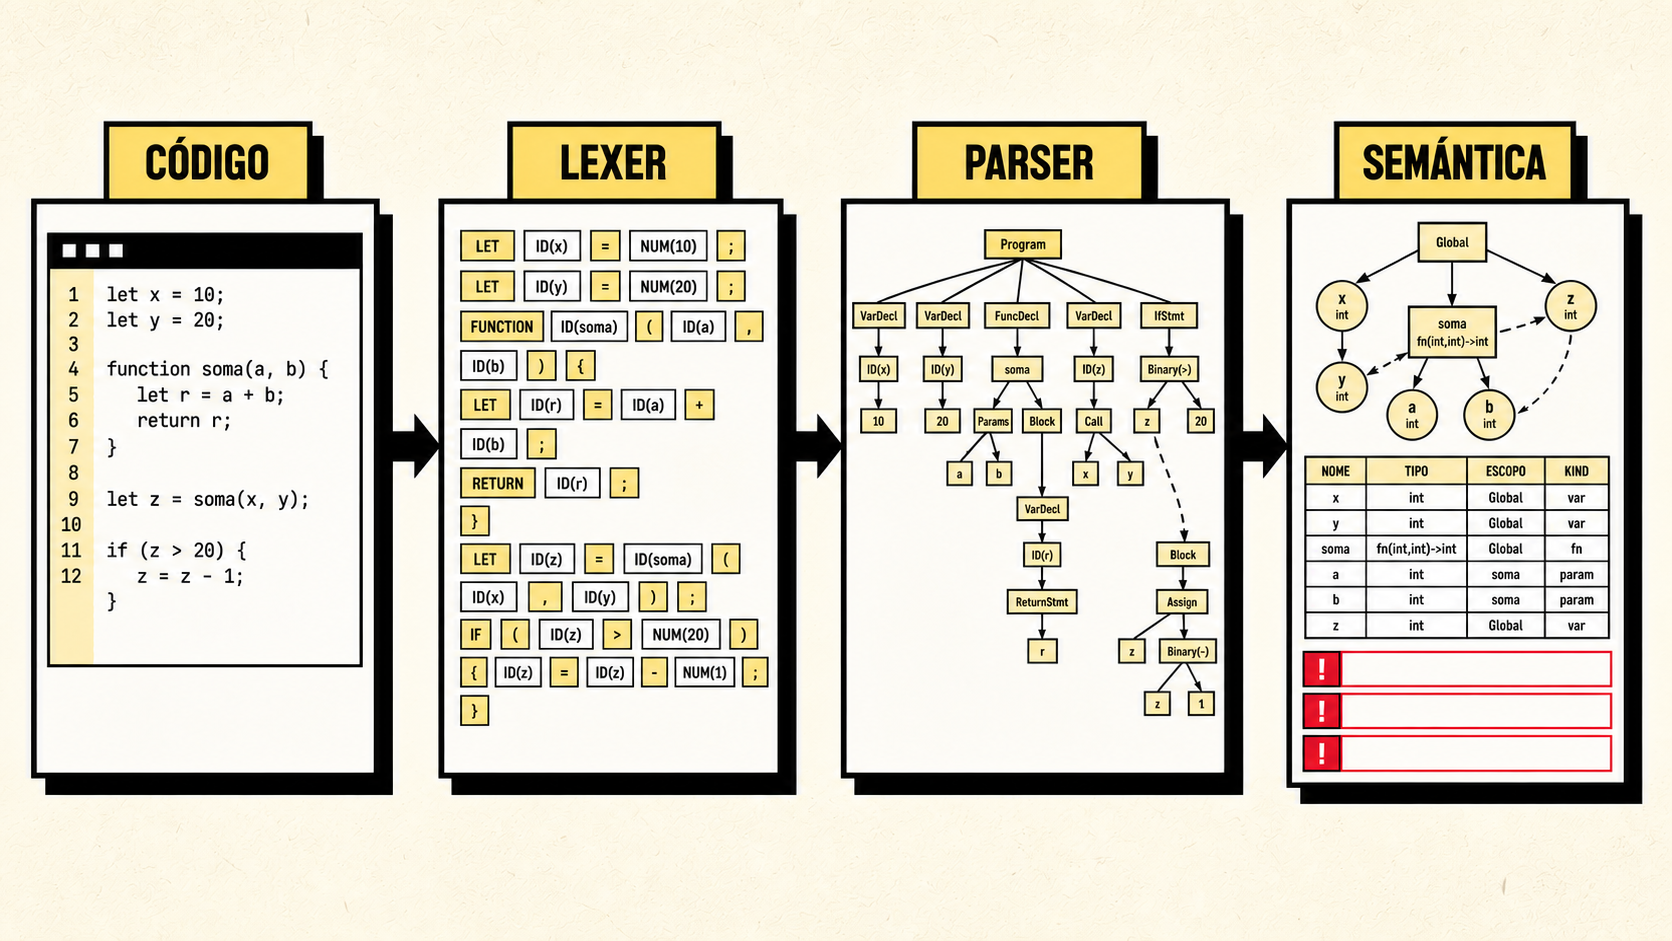
\includegraphics[width=0.84\textwidth]{../../presentation/assets/compiler-pipeline-neobrutalist.png}
  }{
    \fbox{\parbox{0.8\textwidth}{\centering
      Código fuente $\rightarrow$ análisis léxico $\rightarrow$ análisis sintáctico
      $\rightarrow$ análisis semántico}}
  }
  \vfill
  {\large\bfseries Informe técnico, teórico y práctico ampliado\par}
  \vspace{0.55cm}
  {\large Grupo DragonsSlayers 2.0\par}
  \vspace{0.3cm}
  \begin{tabular}{rl}
    Pablo Daniel Barillas Moreno & 22193 \\
    Hugo Daniel Barillas Ajín & 23556 \\
    Ernesto Ascencio & 23009
  \end{tabular}
  \vspace{0.65cm}

  {\large Catedrático: Ing. Carlos Valdéz\par}
  {\large Agosto de 2026\par}
\end{titlepage}
\nopagecolor
\color{black}
\hypersetup{pageanchor=true}

\pagenumbering{roman}

\chapter*{Resumen}
\addcontentsline{toc}{chapter}{Resumen}

Este informe documenta integralmente el diseño y la construcción de
\textbf{Compiscript Semantic IDE}, un entorno académico que integra las tres primeras
fases del frente de un compilador: análisis léxico, análisis sintáctico y análisis
semántico. La entrada es código fuente escrito en \Compiscript, un lenguaje educativo
inspirado en TypeScript. La salida reúne tokens, diagnósticos localizados, árbol de
parseo, árbol semántico anotado, tabla de símbolos, árbol de ámbitos, referencias y
capturas de variables en closures.

El lexer y el parser son generados con \ANTLR{} mediante \archivo{antlr4ts}. La fase
semántica recorre el árbol de parseo con un Visitor escrito en TypeScript. Esta fase
aplica reglas de tipos, resolución de nombres, mutabilidad, funciones, clases,
herencia, arreglos, control de flujo, inicialización y visibilidad. La arquitectura
mantiene una separación estricta entre el motor y sus consumidores: la interfaz
React, la herramienta de línea de comandos y la aplicación Electron utilizan la
misma función de orquestación y el mismo contrato de resultado.

La documentación describe tanto la fundamentación teórica como las decisiones
prácticas. Se detallan la gramática, el sistema de tipos, el modelo de símbolos, los
algoritmos de resolución, el manejo de scopes, la inferencia de retornos, la
identidad de clases, la detección de código inalcanzable, el catálogo
\diag{SEM001}--\diag{SEM023} y el diseño de la experiencia de usuario. También se
presentan diagramas vectoriales, ejemplos reproducibles, una matriz de trazabilidad y
la estrategia de pruebas.

La versión documentada reporta \textbf{115 pruebas aprobadas en 7 suites}, generación
reproducible de ANTLR, comprobación TypeScript y build de producción exitoso con
\textbf{3368 módulos transformados}. El
alcance concluye en el análisis semántico: no se interpreta el programa, no se genera
código intermedio y no se produce código de máquina.

\textbf{Palabras clave:} compiladores, análisis semántico, tabla de símbolos,
\ANTLR, TypeScript, Visitor, ámbitos, sistema de tipos, IDE.

\chapter*{Abstract}
\addcontentsline{toc}{chapter}{Abstract}

This report presents the complete design and implementation of
\textbf{Compiscript Semantic IDE}, an academic environment integrating lexical,
syntactic and semantic analysis. ANTLR-generated recognizers transform source text
into tokens and a concrete parse tree. A TypeScript Visitor then performs name
resolution, type checking, scope management, control-flow validation, class and
function analysis, and semantic-tree construction.

The system exposes a unified result model to a React web interface, a command-line
client and an Electron desktop application. Its semantic infrastructure includes
symbol insertion, lookup, controlled updates, nested scopes, references, closure
captures, class identity, inheritance and return-type inference. The implementation
is validated by 115 automated tests distributed across seven suites (dedicated lexer,
parser and semantic testers, plus rubric regressions). This document
combines theoretical background, implementation details, diagrams, reproducible
examples, traceability and operational instructions.

\tableofcontents
\listoffigures
\listoftables
\clearpage
\pagenumbering{arabic}

\chapter{Introducción}

\section{Planteamiento del problema}

Reconocer que una secuencia de caracteres cumple una gramática es necesario, pero no
suficiente para determinar si un programa tiene sentido. Un parser puede aceptar
\codigo{total = "hola" + verdadero;} si la producción permite una asignación y una
suma; sin embargo, el programa todavía puede violar reglas de tipos, referirse a
identificadores inexistentes o usar una instrucción de control fuera de su contexto.
Estas restricciones dependen de información que no está disponible en una regla
sintáctica aislada.

El Proyecto 1 aborda esa brecha mediante una fase semántica observable. No se trata
solo de emitir una lista de errores: el producto debe explicar qué símbolos existen,
en qué ámbito viven, qué tipo posee cada expresión, cuáles declaraciones son
referenciadas y cómo se relacionan las clases. A la vez, la herramienta debe ser
usable desde una interfaz gráfica y conservar un núcleo suficientemente modular para
pruebas automatizadas.

\section{Justificación}

Construir un analizador semántico obliga a conectar teoría formal con decisiones de
ingeniería de software. La gramática define formas posibles, pero el sistema de tipos
y la tabla de símbolos definen relaciones que atraviesan el árbol completo. Por
ejemplo, comprobar una llamada requiere conocer la firma declarada, resolver el
identificador de la función, analizar todos los argumentos y comparar sus tipos en
orden.

El proyecto permite experimentar con un pipeline generado, hace visibles estructuras
internas de un compilador, transforma requisitos en algoritmos comprobables y
establece una base para interpretación o generación de código.

\section{Objetivo general}

Construir una fase de análisis semántico para \Compiscript{} que sea verificable
mediante pruebas, observable desde un IDE y modular para servir como base de fases
posteriores del compilador.

\section{Objetivos específicos}

\begin{enumerate}
  \item Generar el lexer y parser desde una gramática \ANTLR.
  \item Integrar las fases léxica, sintáctica y semántica mediante un único orquestador.
  \item Diseñar un sistema de tipos para primitivos, arreglos, funciones, clases e instancias.
  \item Implementar inserción, recuperación, actualización y manejo de ámbitos.
  \item Validar declaraciones, expresiones, llamadas, retornos, clases y control.
  \item Registrar referencias y variables capturadas por funciones anidadas.
  \item Construir un árbol semántico anotado y métricas de la fase.
  \item Presentar tokens, árboles, símbolos y diagnósticos en una interfaz amigable.
  \item Mantener ejemplos de aceptación y rechazo junto con pruebas de regresión.
  \item Documentar arquitectura, decisiones, instalación y trazabilidad.
\end{enumerate}

\section{Alcance}

El sistema recibe texto o un archivo \archivo{.cps}; genera tokens; valida la
estructura; ejecuta reglas semánticas cuando las fases anteriores son válidas; y
presenta resultados en web, CLI o escritorio. Se incluyen declaraciones, tipos,
arreglos, funciones, closures, clases, herencia, acceso a miembros, condicionales,
ciclos, \codigo{switch}, \codigo{try/catch}, \codigo{break}, \codigo{continue} y
\codigo{return}.

Quedan fuera del alcance la ejecución de instrucciones, generación de representación
intermedia, optimización, generación de máquina, enlazado externo y módulos.

\section{Metodología de desarrollo}

El trabajo siguió un ciclo incremental. Primero se alineó la gramática y se regeneró
ANTLR. Después se diseñaron tipos, símbolos y ámbitos. Las reglas se incorporaron por
familias y cada una recibió casos válidos, inválidos y regresiones. Finalmente se
integró el resultado en la UI, se elaboraron ejemplos y se auditó la consistencia.

\begin{figure}[H]
\centering
\setlength{\unitlength}{1mm}
\begin{picture}(150,42)
  \put(2,27){\framebox(27,10){Requisito}}
  \put(40,27){\framebox(27,10){Diseño}}
  \put(78,27){\framebox(30,10){Implementación}}
  \put(119,27){\framebox(27,10){Prueba}}
  \put(98,5){\framebox(28,10){Auditoría}}
  \put(56,5){\framebox(31,10){Documentación}}
  \put(29,32){\vector(1,0){11}}
  \put(67,32){\vector(1,0){11}}
  \put(108,32){\vector(1,0){11}}
  \put(133,27){\vector(-1,-1){17}}
  \put(98,10){\vector(-1,0){11}}
  \put(56,10){\line(-1,0){42}}
  \put(14,10){\vector(0,1){17}}
\end{picture}
\caption{Ciclo incremental aplicado a cada familia de reglas.}
\label{fig:metodologia}
\end{figure}

\chapter{Fundamentos teóricos}

\section{El frente de un compilador}

El frente transforma texto en una representación estructurada y enriquecida.
El lexer agrupa caracteres; el parser comprueba derivaciones; y el análisis semántico
relaciona declaraciones y usos, calcula tipos y aplica restricciones contextuales.

\begin{figure}[H]
\centering
\setlength{\unitlength}{1mm}
\begin{picture}(150,42)
  \put(2,26){\framebox(30,11){\shortstack{Código\\fuente}}}
  \put(41,26){\framebox(27,11){Lexer}}
  \put(77,26){\framebox(27,11){Parser}}
  \put(113,26){\framebox(34,11){\shortstack{Visitor\\semántico}}}
  \put(43,4){\framebox(23,9){Tokens}}
  \put(79,4){\framebox(23,9){CST}}
  \put(116,4){\framebox(29,9){\shortstack{Modelo\\semántico}}}
  \put(32,31){\vector(1,0){9}}
  \put(68,31){\vector(1,0){9}}
  \put(104,31){\vector(1,0){9}}
  \put(55,26){\vector(0,-1){13}}
  \put(91,26){\vector(0,-1){13}}
  \put(130,26){\vector(0,-1){13}}
\end{picture}
\caption{Transformaciones principales del frente implementado.}
\label{fig:front-end}
\end{figure}

\section{Tokens, lexemas y posiciones}

Un lexema es el fragmento concreto de entrada; un token es su categoría. En
\codigo{let total: integer = 5;}, \codigo{total} y \codigo{5} son lexemas, mientras
\codigo{Identifier} e \codigo{IntegerLiteral} son tokens. Cada token conserva línea y
columna; los símbolos guardan declaración y referencias; y los diagnósticos se
vinculan a la construcción que los originó.

\section{Gramáticas libres de contexto}

Una gramática puede expresarse como \(G=(V,\Sigma,P,S)\), donde \(V\) es el conjunto
de no terminales, \(\Sigma\) el de terminales, \(P\) las producciones y \(S\) el
símbolo inicial. \codigo{program} es la regla inicial. ANTLR 4 utiliza predicción
adaptativa LL(*) y genera un parser descendente; el proyecto no implementa tablas
\codigo{ACTION/GOTO}.

\section{CST, AST y árbol semántico}

El CST conserva reglas auxiliares, puntuación y terminales. Un AST elimina detalles
superficiales. Este proyecto mantiene el CST para trazabilidad y construye un árbol
semántico anotado para explicar tipos, símbolos y diagnósticos.

\begin{table}[H]
\centering
\begin{tabularx}{\textwidth}{lYY}
\toprule
Representación & Contenido & Uso \\
\midrule
CST & reglas y terminales de ANTLR & validación sintáctica y depuración \\
Árbol semántico & nodos conceptuales, tipos y símbolos & explicación y UI \\
Tabla de símbolos & declaraciones, firmas y referencias & resolución contextual \\
\bottomrule
\end{tabularx}
\caption{Representaciones internas complementarias.}
\end{table}

\section{Atributos y análisis semántico}

La semántica puede verse como el cálculo de atributos. Una expresión sintetiza su
tipo a partir de sus hijos y una instrucción hereda el ámbito y el contexto:
\[
\frac{\Gamma\vdash e_1:T_1 \quad \Gamma\vdash e_2:T_2
      \quad \operatorname{sumable}(T_1,T_2)}
     {\Gamma\vdash e_1+e_2:\operatorname{resultado}(T_1,T_2)}.
\]
\(\Gamma\) es el entorno de símbolos visible.

\section{Tabla de símbolos y resolución}

La resolución de un nombre \(n\) desde un ámbito \(s\) se define como:
\[
\operatorname{resolve}(n,s)=
\begin{cases}
\operatorname{local}(n,s), & n\in s,\\
\operatorname{resolve}(n,\operatorname{parent}(s)), & parent(s)\neq\varnothing,\\
\bot, & \text{en otro caso}.
\end{cases}
\]
\(\bot\) produce \diag{SEM001}. La redeclaración consulta solo el ámbito actual; por
ello se permite shadowing en ámbitos hijos.

\section{Sistemas de tipos}

Un tipo resume operaciones válidas. El proyecto combina clases nominales con arreglos
y funciones estructurados. \codigo{unknown} representa información todavía no
inferida y \codigo{error} absorbe consecuencias después de un diagnóstico. Se admite
\(\codigo{integer}\preceq\codigo{float}\), pero no la conversión implícita inversa.

\section{Flujo de control}

El análisis distingue terminación del camino actual y retorno garantizado. Para un
condicional completo:
\[
\operatorname{returns}(if(e)\ B_1\ else\ B_2)
=\operatorname{returns}(B_1)\land\operatorname{returns}(B_2).
\]
Una instrucción posterior a \codigo{return}, \codigo{break} o \codigo{continue} en el
mismo bloque es inalcanzable.

\section{Patrón Visitor}

El Visitor separa la estructura generada del comportamiento. La implementación no
modifica el parser producido por ANTLR, por lo que la regeneración continúa siendo
reproducible y las reglas semánticas permanecen en módulos TypeScript propios.

\chapter{Especificación de Compiscript}

\section{Fuentes de verdad}

La definición se construyó con el README, la gramática
\archivo{src/grammars/Compiscript.g4} y el enunciado semántico. La gramática gobierna
la sintaxis; el enunciado las validaciones; y los ejemplos aclaran intención cuando
no contradicen las fuentes anteriores.

\begin{resumenclave}
Los archivos de \archivo{src/generated} no se editan. Se modifica
\archivo{Compiscript.g4} y se ejecuta \codigo{npm run generate}.
\end{resumenclave}

\section{Unidades léxicas}

\begin{longtable}{p{0.22\textwidth}p{0.68\textwidth}}
\caption{Categorías léxicas principales.}\label{tab:lexico}\\
\toprule
Categoría & Elementos representativos \\
\midrule
\endfirsthead
\toprule
Categoría & Elementos representativos \\
\midrule
\endhead
Declaraciones & \codigo{let}, \codigo{var}, \codigo{const}, \codigo{function}, \codigo{class} \\
Control & \codigo{if}, \codigo{else}, \codigo{while}, \codigo{for}, \codigo{foreach}, \codigo{switch} \\
Transferencia & \codigo{return}, \codigo{break}, \codigo{continue} \\
Objetos & \codigo{new}, \codigo{this} \\
Tipos & \codigo{boolean}, \codigo{integer}, \codigo{float}, \codigo{string} \\
Literales & enteros, decimales, cadenas, booleanos y \codigo{null} \\
Operadores & aritméticos, lógicos, relacionales, igualdad, asignación y ternario \\
Separadores & paréntesis, llaves, corchetes, coma, punto, dos puntos y punto y coma \\
Ignorados & espacios, saltos de línea y comentarios \\
\bottomrule
\end{longtable}

\section{Declaraciones}

\begin{verbatim}
let contador: integer = 0;
var promedio: float = 87.5;
const NOMBRE: string = "Compiscript";
let activo: boolean = true;

function sumar(a: integer, b: integer): integer {
  return a + b;
}
\end{verbatim}

\section{Expresiones y precedencia}

De menor a mayor prioridad aparecen asignación, ternario, OR, AND, igualdad,
relacionales, suma/resta, multiplicación/división/módulo, unarios y primarias.

\begin{figure}[H]
\centering
\setlength{\unitlength}{1mm}
\begin{picture}(150,76)
  \put(45,66){\framebox(60,8){Asignación}}
  \put(45,55){\framebox(60,8){Ternario}}
  \put(45,44){\framebox(60,8){OR y AND}}
  \put(45,33){\framebox(60,8){Igualdad y relacionales}}
  \put(45,22){\framebox(60,8){Suma y resta}}
  \put(45,11){\framebox(60,8){Multiplicación, división y módulo}}
  \put(45,0){\framebox(60,8){Unarias, sufijos y primarias}}
  \put(75,66){\vector(0,-1){3}}
  \put(75,55){\vector(0,-1){3}}
  \put(75,44){\vector(0,-1){3}}
  \put(75,33){\vector(0,-1){3}}
  \put(75,22){\vector(0,-1){3}}
  \put(75,11){\vector(0,-1){3}}
\end{picture}
\caption{Jerarquía de precedencia; la prioridad aumenta hacia abajo.}
\label{fig:precedencia}
\end{figure}

\section{Control, funciones, clases y arreglos}

Se soportan condicionales, ciclos, \codigo{foreach}, \codigo{switch} y
\codigo{try/catch}. La gramática activa exige bloques con llaves. Las funciones
pueden ser recursivas o anidadas. Las clases admiten herencia, \codigo{this},
constructor y miembros. Los arreglos pueden ser multidimensionales.

\begin{verbatim}
class Caja {
  let valor: integer;
  function constructor(valor: integer) {
    this.valor = valor;
  }
  function obtener(): integer {
    return this.valor;
  }
}
let cajas: Caja[] = [new Caja(10), new Caja(20)];
print(cajas[0].obtener());
\end{verbatim}

\section{Decisiones interpretativas}

\codigo{float} se añadió porque el requisito semántico lo exige. Se incorporaron tipo,
literal decimal y promoción segura. Para \codigo{switch}, se adoptó un discriminante
escalar y casos comparables, coherente con la gramática y los ejemplos oficiales.

\chapter{Arquitectura general}

\section{Capas}

\begin{figure}[H]
\centering
\setlength{\unitlength}{1mm}
\begin{picture}(150,65)
  \put(15,54){\framebox(120,9){React IDE \hspace{9mm} CLI \hspace{9mm} Electron}}
  \put(15,41){\framebox(120,9){Orquestación: src/lib/analyze.ts}}
  \put(15,28){\framebox(120,9){ANTLR: lexer, token stream, parser y CST}}
  \put(15,15){\framebox(120,9){Semántica: scopes, tipos, flujo y diagnósticos}}
  \put(15,2){\framebox(120,9){Gramática, ejemplos, pruebas y documentación}}
  \put(75,54){\vector(0,-1){4}}
  \put(75,41){\vector(0,-1){4}}
  \put(75,28){\vector(0,-1){4}}
  \put(75,15){\vector(0,-1){4}}
\end{picture}
\caption{Arquitectura por capas.}
\label{fig:layers}
\end{figure}

\section{Organización del repositorio}

\begin{verbatim}
compiscript-ide-work/
|-- docs/                 documentación e informe
|-- electron/main.cjs     proceso de escritorio
|-- examples/             casos léxicos, sintácticos y semánticos
|-- presentation/         presentación e imágenes
|-- public/               recursos del frontend
|-- src/
|   |-- __tests__/        siete suites Vitest
|   |-- cli/run.ts        cliente de consola
|   |-- generated/        salida de ANTLR
|   |-- grammars/         gramática fuente
|   |-- lib/              orquestación
|   |-- semantic/         fase semántica
|   +-- ui/               aplicación React
|-- package.json
|-- tsconfig.json
+-- vite.config.ts
\end{verbatim}

\section{Pipeline de ejecución}

\begin{figure}[H]
\centering
\setlength{\unitlength}{1mm}
\begin{picture}(150,62)
  \put(2,43){\framebox(22,9){Entrada}}
  \put(33,43){\framebox(28,9){Lexer + fill}}
  \put(70,43){\framebox(28,9){¿modo lexer?}}
  \put(70,23){\framebox(28,9){Parser}}
  \put(107,23){\framebox(33,9){¿sin errores?}}
  \put(108,43){\framebox(31,9){Resultado lexer}}
  \put(70,3){\framebox(30,9){Visitors}}
  \put(112,3){\framebox(33,9){AnalyzeResult}}
  \put(24,47){\vector(1,0){9}}
  \put(61,47){\vector(1,0){9}}
  \put(84,43){\vector(0,-1){11}}
  \put(98,47){\vector(1,0){10}}
  \put(98,27){\vector(1,0){9}}
  \put(123,23){\vector(-1,-1){23}}
  \put(100,7){\vector(1,0){12}}
  \put(140,27){\line(1,0){7}}
  \put(147,27){\vector(0,-1){15}}
\end{picture}
\caption{Decisiones del orquestador.}
\label{fig:runtime}
\end{figure}

\section{Contrato de resultado}

\archivo{AnalyzeResult} contiene tokens, errores, tres representaciones del CST,
resultado semántico, explicación y resumen:
\[
\operatorname{accepted}=
\neg E_{\mathrm{lex}}\land\neg E_{\mathrm{syn}}\land
\left(m\neq\mathrm{semantic}\lor\neg E_{\mathrm{sem}}\right).
\]
Las advertencias no rechazan el archivo.

\begin{figure}[H]
\centering
\setlength{\unitlength}{1mm}
\begin{picture}(150,48)
  \put(55,19){\framebox(40,10){AnalyzeResult}}
  \put(5,35){\framebox(30,9){tokens}}
  \put(60,35){\framebox(30,9){errores}}
  \put(115,35){\framebox(30,9){CST}}
  \put(5,2){\framebox(30,9){semántica}}
  \put(60,2){\framebox(30,9){resumen}}
  \put(115,2){\framebox(30,9){explicación}}
  \put(60,29){\vector(-2,1){25}}
  \put(75,29){\vector(0,1){6}}
  \put(90,29){\vector(2,1){25}}
  \put(60,19){\vector(-2,-1){25}}
  \put(75,19){\vector(0,-1){8}}
  \put(90,19){\vector(2,-1){25}}
\end{picture}
\caption{Contrato serializable común.}
\label{fig:result-model}
\end{figure}

\section{Tecnologías}

\begin{table}[H]
\centering
\begin{tabularx}{\textwidth}{l l Y}
\toprule
Tecnología & Versión & Responsabilidad \\
\midrule
TypeScript & 5.6 & motor y UI tipados \\
ANTLR / antlr4ts & 4 / 0.5 alpha & lexer, parser, listener y Visitor \\
React & 19 & interfaz declarativa \\
Vite & 6 & desarrollo y build web \\
Vitest & 3.2 & pruebas \\
Electron & 43 & escritorio \\
electron-builder & 26 & empaquetado Windows, macOS y Linux \\
LaTeX + TikZ & TeX Live & documentación vectorial \\
\bottomrule
\end{tabularx}
\caption{Dependencias tecnológicas principales.}
\end{table}

\section{Recursos visuales de referencia}

\begin{figure}[H]
  \centering
  \IfFileExists{../../presentation/assets/compiler-pipeline-neobrutalist.png}{
    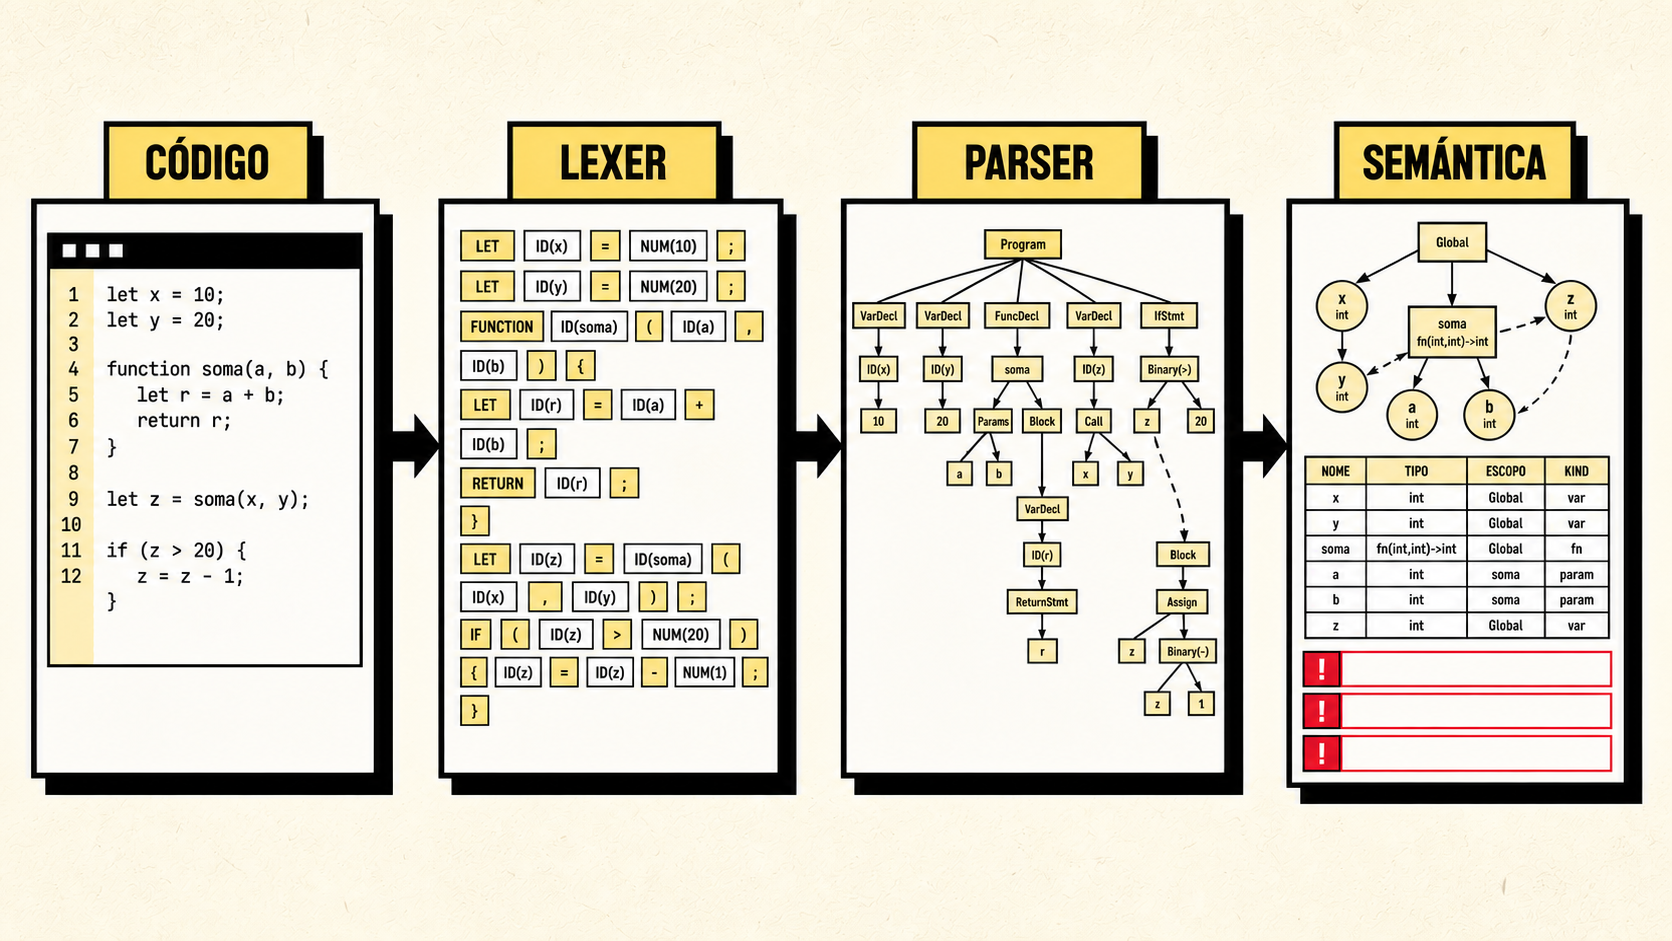
\includegraphics[width=0.9\textwidth]{../../presentation/assets/compiler-pipeline-neobrutalist.png}
  }{\fbox{\parbox{0.85\textwidth}{Imagen del pipeline no encontrada.}}}
  \caption{Referencia visual neobrutalista del pipeline de Compiscript.}
  \label{fig:pipeline-hero}
\end{figure}

\begin{figure}[H]
  \centering
  \IfFileExists{../../presentation/assets/scopes-symbol-table-neobrutalist.png}{
    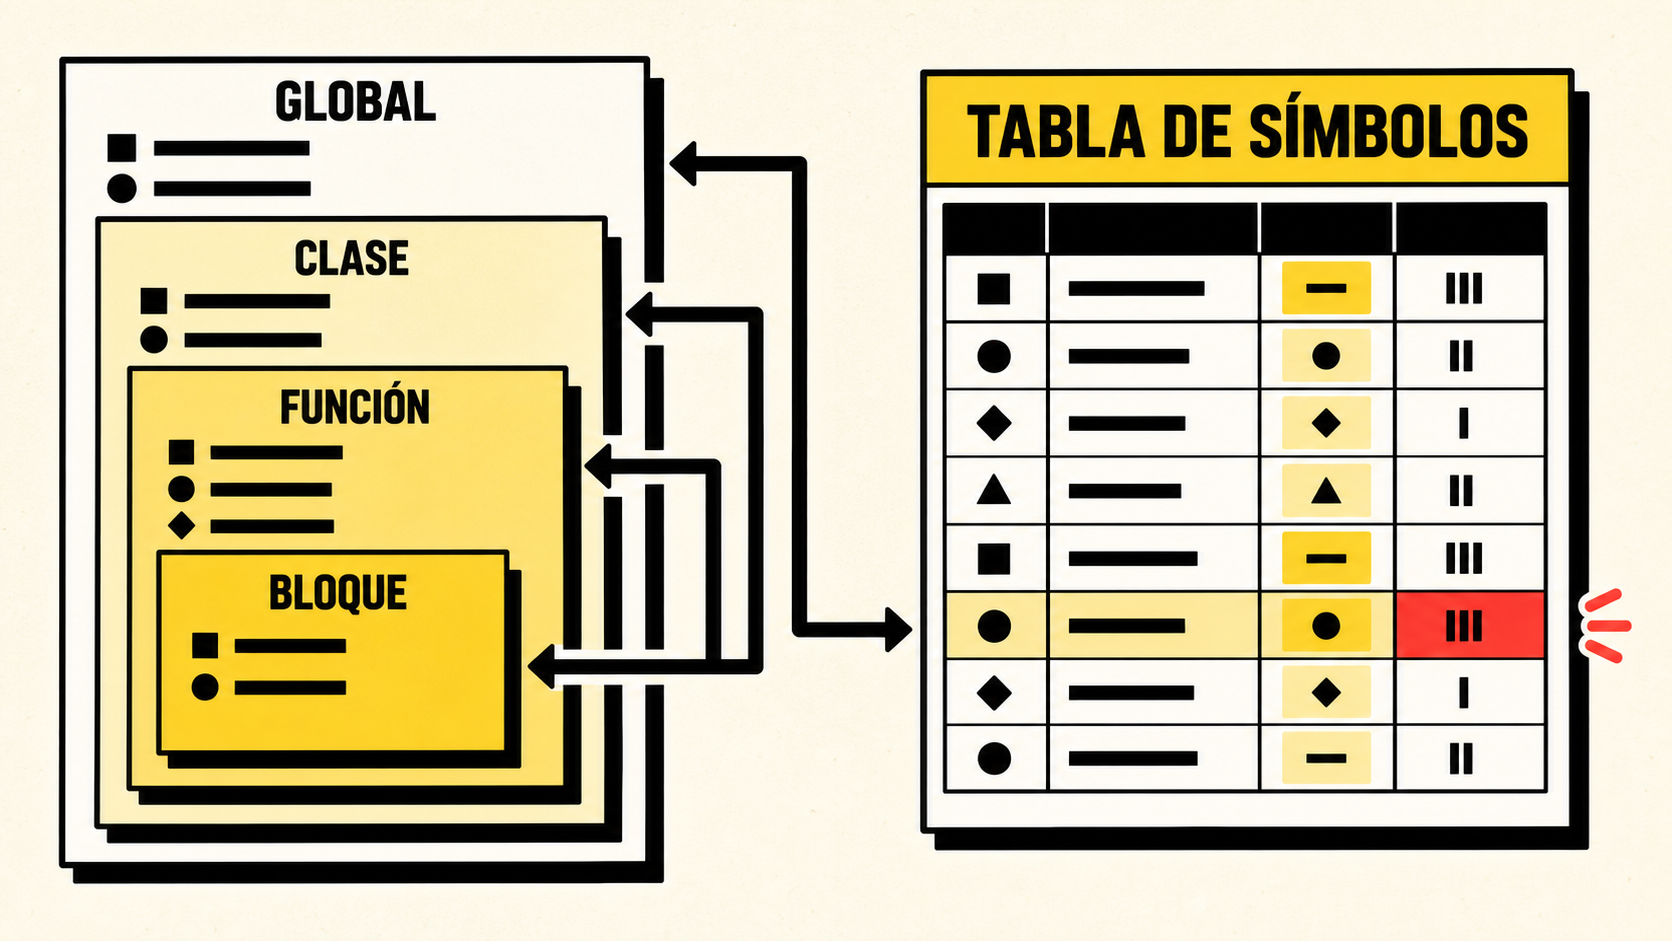
\includegraphics[width=0.88\textwidth]{../../presentation/assets/scopes-symbol-table-neobrutalist.png}
  }{\fbox{\parbox{0.85\textwidth}{Imagen de ámbitos no encontrada.}}}
  \caption{Referencia visual neobrutalista de ámbitos y tabla de símbolos.}
  \label{fig:scopes-image}
\end{figure}

Ambas piezas siguen la identidad visual neobrutalista de la interfaz vigente:
fondos crema, superficies blancas y amarillas, bordes negros gruesos, esquinas
rectas y sombras sólidas desplazadas. Funcionan como referencias conceptuales para
explicar el sistema; no sustituyen las capturas ni los resultados producidos por una
ejecución real del IDE.

\chapter{Implementación léxica y sintáctica}

\section{Generación con ANTLR}

El script \codigo{npm run generate} invoca \archivo{antlr4ts-cli} con generación de
listener y Visitor. La salida se deposita en \archivo{src/generated}; incluye lexer,
parser, interfaces y archivos auxiliares de vocabulario. La gramática permanece como
fuente declarativa y el código generado puede reproducirse.

\begin{verbatim}
antlr4ts -Xexact-output-dir -visitor -listener
  -o src/generated src/grammars/Compiscript.g4
\end{verbatim}

Nunca se corrige un defecto editando \archivo{CompiscriptParser.ts}. Se modifica
\archivo{Compiscript.g4}, se regenera y se ejecuta toda la suite.

\section{Integración del lexer}

\codigo{ANTLRInputStream} adapta el texto; \codigo{CompiscriptLexer} reconoce tokens;
y \codigo{CommonTokenStream} almacena el resultado. \codigo{tokenStream.fill()} obliga
al lexer a recorrer toda la entrada antes del parser. Así se recolectan múltiples
errores léxicos y se conservan tokens posteriores.

\begin{longtable}{p{0.24\textwidth}p{0.66\textwidth}}
\toprule
Campo & Significado \\
\midrule
\endhead
\codigo{index} & posición dentro del token stream \\
\codigo{type} & identificador numérico generado \\
\codigo{typeName} & nombre simbólico del vocabulario \\
\codigo{text} & lexema exacto \\
\codigo{line} & línea base uno \\
\codigo{column} & columna convertida a base uno \\
\codigo{channel} & canal del token \\
\bottomrule
\caption{Información serializada de un token.}
\end{longtable}

\section{Normalización de errores léxicos}

El listener predeterminado fue sustituido por \archivo{CollectingErrorListener}. En
lugar de escribir en consola, construye objetos localizables y traduce los mensajes.
Fragmentos contiguos se agrupan: \codigo{@@@} produce un diagnóstico con ese símbolo,
no tres mensajes equivalentes.

Las cadenas reciben tratamiento específico. Una comilla sin cierre produce una
descripción de cadena incompleta; una secuencia de escape no permitida genera otro
mensaje. La normalización conserva el fragmento ofensivo.

\section{Integración del parser}

Después de inspeccionar el token stream se ejecuta \codigo{seek(0)}. El parser agrega
el listener recolector, habilita el árbol y llama \codigo{program()}.

\begin{verbatim}
tokenStream.seek(0);
const parser = new CompiscriptParser(tokenStream);
parser.errorHandler = new DefaultErrorStrategy();
parser.buildParseTree = true;
const tree = parser.program();
\end{verbatim}

\codigo{DefaultErrorStrategy} puede insertar conceptualmente un token faltante,
eliminar uno sobrante o sincronizarse con una regla posterior. El objetivo es evitar
que una anomalía impida localizar problemas independientes.

\section{Filtrado de cascadas}

Cuando el lexer descarta un símbolo, el parser puede informar una consecuencia en la
misma posición. El orquestador filtra únicamente errores sintácticos inmediatamente
cercanos al fragmento léxico. Para cadenas inválidas se admite una única consecuencia
en la línea siguiente.

\begin{figure}[H]
\centering
\setlength{\unitlength}{1mm}
\begin{picture}(150,42)
  \put(3,28){\framebox(35,9){Errores ANTLR}}
  \put(57,28){\framebox(38,9){Traducir y ubicar}}
  \put(113,28){\framebox(32,9){Especializar}}
  \put(108,4){\framebox(38,9){Agrupar y deduplicar}}
  \put(56,4){\framebox(34,9){Filtrar cascadas}}
  \put(3,4){\framebox(35,9){Diagnósticos UI}}
  \put(38,32){\vector(1,0){19}}
  \put(95,32){\vector(1,0){18}}
  \put(129,28){\vector(0,-1){15}}
  \put(108,8){\vector(-1,0){18}}
  \put(56,8){\vector(-1,0){18}}
\end{picture}
\caption{Normalización de diagnósticos léxicos y sintácticos.}
\label{fig:syntax-errors}
\end{figure}

\section{Representaciones del árbol}

El CST se conserva como salida Lisp original, recorrido indentado y nodos recursivos
para la vista interactiva. La conversión recorre el objeto \archivo{ParseTree}; no
reinterpreta la cadena Lisp, porque tokens como paréntesis la harían ambigua.

\section{Transición a semántica}

La fase semántica solo recibe un CST sin errores previos. Un nodo insertado por
recuperación puede carecer de identificador o expresión real y generaría mensajes
semánticos falsos. El resultado distingue \codigo{not-requested}, \codigo{skipped} y
\codigo{completed}.

\chapter{Modelo semántico}

\section{Visión general}

La fase coopera con un administrador de ámbitos, un registro de clases, un sistema de
tipos, un catálogo de diagnósticos y análisis de flujo.

\begin{figure}[H]
\centering
\setlength{\unitlength}{1mm}
\begin{picture}(150,50)
  \put(2,20){\framebox(25,10){CST válido}}
  \put(36,20){\framebox(27,10){Prepasada}}
  \put(72,20){\framebox(24,10){Visitor}}
  \put(72,38){\framebox(24,8){Tipos}}
  \put(72,3){\framebox(24,8){Flujo}}
  \put(105,20){\framebox(25,10){\shortstack{Scopes y\\símbolos}}}
  \put(136,20){\framebox(14,10){Árbol}}
  \put(27,25){\vector(1,0){9}}
  \put(63,25){\vector(1,0){9}}
  \put(84,38){\vector(0,-1){8}}
  \put(84,11){\vector(0,1){9}}
  \put(96,25){\vector(1,0){9}}
  \put(130,25){\vector(1,0){6}}
\end{picture}
\caption{Colaboración de módulos semánticos.}
\label{fig:semantic-modules}
\end{figure}

\section{Prepasada y hoisting local}

Clases y funciones deben ser visibles antes de su aparición textual para permitir
recursión y referencias adelantadas. Las declaraciones se registran antes de recorrer
instrucciones ordinarias del mismo scope. El hoisting es local: una función anidada no
se convierte en global.

La prepasada asigna identidad a clases, vincula herencia y prepara miembros. El
Visitor entra después en cada cuerpo. Esta división separa descubrimiento y
validación.

\section{Árbol semántico anotado}

\archivo{SemanticTreeNode} contiene ID, clase de nodo, etiqueta, ubicación, tipo
opcional, símbolo opcional, diagnósticos e hijos. No es una IR ejecutable; es una
proyección pedagógica que conecta CST y significado.

\section{Límite y deduplicación}

El Visitor limita la salida a 500 diagnósticos semánticos. La creación centralizada
asigna ID, severidad e información relacionada. Los tipos \codigo{unknown} y
\codigo{error} reducen cascadas posteriores.

\chapter{Sistema de tipos}

\section{Representación}

\archivo{SemanticType} es una unión discriminada. Los primitivos incluyen
\codigo{boolean}, \codigo{integer}, \codigo{float}, \codigo{string},
\codigo{null}, \codigo{void}, \codigo{unknown} y \codigo{error}. Arreglos, funciones,
clases e instancias contienen estructura adicional.

\begin{table}[H]
\centering
\begin{tabularx}{\textwidth}{lY}
\toprule
Tipo & Información almacenada \\
\midrule
Primitivo & nombre canónico \\
Arreglo & tipo de elemento y dimensiones \\
Función & parámetros y retorno \\
Clase & nombre e identidad de declaración \\
Instancia & clase asociada e identidad \\
\codigo{unknown} & inferencia pendiente \\
\codigo{error} & causa ya diagnosticada \\
\bottomrule
\end{tabularx}
\caption{Familias del modelo de tipos.}
\end{table}

\section{Igualdad y asignabilidad}

\archivo{typesEqual} compara estructura e identidad. Dos clases homónimas en ámbitos
distintos no son iguales. \archivo{isAssignable} incorpora igualdad, promoción
numérica, \codigo{null} donde aplica e herencia.

\begin{figure}[H]
\centering
\setlength{\unitlength}{1mm}
\begin{picture}(150,42)
  \put(12,27){\framebox(27,9){integer}}
  \put(62,27){\framebox(27,9){float}}
  \put(12,6){\framebox(27,9){string}}
  \put(62,6){\framebox(27,9){boolean}}
  \put(111,27){\framebox(28,9){unknown}}
  \put(111,6){\framebox(28,9){error}}
  \put(39,31){\vector(1,0){23}}
  \put(44,33){\makebox(14,5){\scriptsize promoción}}
  \put(125,27){\vector(0,-1){12}}
  \put(126,18){\makebox(20,5){\scriptsize absorción}}
\end{picture}
\caption{Relaciones destacadas del sistema de tipos.}
\label{fig:type-relations}
\end{figure}

\section{Operadores aritméticos}

\codigo{numericResult} devuelve \codigo{float} si algún operando es decimal; en otro
caso devuelve \codigo{integer}. La suma admite concatenación cuando ambos operandos
son cadenas. Aplicar aritmética a categorías inválidas produce \diag{SEM004}.

\begin{table}[H]
\centering
\begin{tabular}{lll}
\toprule
Izquierdo & Derecho & Resultado \\
\midrule
integer & integer & integer \\
integer & float & float \\
float & integer & float \\
float & float & float \\
string & string, solo suma & string \\
\bottomrule
\end{tabular}
\caption{Resultados aritméticos válidos.}
\end{table}

\section{Lógicos, relacionales y comparación}

Los operadores lógicos requieren booleanos. Las comparaciones de orden requieren
números compatibles. Igualdad y desigualdad utilizan \archivo{isComparable}, que
considera igualdad, promoción, \codigo{null} y jerarquía. Toda comparación válida
resulta \codigo{boolean}.

\section{Asignación e inicialización}

Una variable anotada adopta ese tipo y el inicializador debe ser asignable. Sin
anotación, se infiere desde el valor. Una variable sin inicializador queda pendiente;
usarla produce \diag{SEM023}. Las constantes son inmutables.

\begin{verbatim}
let entero: integer = 4;
let decimal: float = entero;
let pendiente: integer;
print(pendiente);          // SEM023
pendiente = 10;
print(pendiente);          // valido
\end{verbatim}

\section{Arreglos}

Un literal analiza todos sus elementos y calcula \archivo{commonType}. Si no existe
tipo compatible se produce \diag{SEM017}. Acceder exige receptor arreglo e índice
entero: un índice decimal produce \diag{SEM015}; indexar un escalar,
\diag{SEM016}.

\section{Funciones y retorno}

Una firma conserva parámetros y retorno. Sin anotación, cada \codigo{return} aporta
un tipo observado y al finalizar se calcula un tipo común. Sin retornos con valor, el
resultado es \codigo{void}. Una anotación incompatible produce \diag{SEM008}.

\section{Clases e identidad}

La igualdad nominal usa \codigo{classId}, no solo nombre. Dos clases
\codigo{Local} en bloques hermanos son tipos distintos. La identidad permite recorrer
herencia y asignar una instancia hija a una variable del padre.

\chapter{Tabla de símbolos y ámbitos}

\section{Modelo de símbolo}

Cada \archivo{SymbolEntry} contiene ID, nombre, categoría, tipo, mutabilidad, scope,
declaración, inicialización, referencias y captura. Funciones agregan firma; clases y
miembros conservan identidad.

\begin{longtable}{p{0.26\textwidth}p{0.64\textwidth}}
\caption{Campos conceptuales de un símbolo.}\label{tab:symbol-entry}\\
\toprule
Campo & Propósito \\
\midrule
\endfirsthead
\toprule
Campo & Propósito \\
\midrule
\endhead
ID & identidad estable \\
Nombre & texto sujeto a resolución \\
Categoría & variable, constante, parámetro, función, clase, campo o método \\
Tipo & declarado o inferido \\
Mutabilidad & controla reasignación \\
Scope ID & entorno propietario \\
Declaración & línea y columna originales \\
Inicialización & uso antes de valor \\
Referencias & ubicaciones de uso \\
Captura & uso desde una función anidada \\
Firma/miembros & metadatos compuestos \\
\bottomrule
\end{longtable}

\section{Ámbitos}

\archivo{ScopeKind} distingue \codigo{global}, \codigo{block},
\codigo{function}, \codigo{class}, \codigo{loop}, \codigo{catch} y
\codigo{switch}. Cada scope conoce padre, hijos, nombre, límites y símbolos.

\begin{figure}[H]
\centering
\setlength{\unitlength}{1mm}
\begin{picture}(150,63)
  \put(58,51){\framebox(34,9){global}}
  \put(7,30){\framebox(35,9){class Caja}}
  \put(55,30){\framebox(40,9){function ejecutar}}
  \put(111,30){\framebox(32,9){block if}}
  \put(7,5){\framebox(38,9){function obtener}}
  \put(53,5){\framebox(38,9){function sumar}}
  \put(105,5){\framebox(35,9){loop for}}
  \put(65,51){\vector(-2,-1){30}}
  \put(75,51){\vector(0,-1){12}}
  \put(85,51){\vector(2,-1){30}}
  \put(24,30){\vector(0,-1){16}}
  \put(68,30){\vector(0,-1){16}}
  \put(82,30){\vector(2,-1){28}}
\end{picture}
\caption{Ejemplo de árbol de ámbitos.}
\label{fig:scope-tree}
\end{figure}

\section{Insertar, recuperar y actualizar}

\codigo{declare} consulta el scope activo; una colisión permite emitir
\diag{SEM002}. \codigo{resolveCurrent} limita la búsqueda; \codigo{resolve} recorre
padres. \codigo{updateSymbol} permite cambiar tipo, firma, inicialización, captura y
referencias, pero preserva identidad, nombre, scope y declaración.

\section{Entrada y salida}

\codigo{enterScope} crea un hijo y lo activa. \codigo{exitScope} fija su final y
restaura el padre. La UI conserva scopes terminados:
\[
S_0=[global],\quad enter(k)\Rightarrow S_{i+1}=S_i\cdot k,\quad
exit\Rightarrow S_{i+1}=parent(top(S_i)).
\]

\section{Shadowing}

Un hijo puede repetir el nombre de un padre. Dentro del hijo se resuelve la entidad
más cercana; al salir vuelve la del padre. Ambas conservan IDs y referencias
independientes.

\section{Referencias}

Cada resolución registra la ubicación del uso, incluso clases en \codigo{new}, campos
y métodos. Esto habilita métricas y una futura navegación a declaración.

\section{Closures}

Si una función anidada resuelve un símbolo de una función externa, se marca
\codigo{captured}. Una variable global no se clasifica como captura.

\begin{verbatim}
function crearContador(): integer {
  let base: integer = 40;
  function incrementar(): integer {
    return base + 1;
  }
  return incrementar();
}
\end{verbatim}

\chapter{Reglas semánticas por construcción}

\section{Declaraciones de variables}

El Visitor analiza primero la anotación y el inicializador. Si ambos existen, verifica
asignabilidad; si solo hay inicializador, infiere; si solo hay anotación, registra la
variable como no inicializada. Finalmente llama \codigo{declare}. Este orden permite
que la entrada final conserve el tipo más útil incluso cuando se reporta un error.

Una redeclaración en el mismo scope produce \diag{SEM002} y agrega información sobre
la ubicación original. Declarar el mismo nombre en un hijo es shadowing válido.

\section{Constantes}

La gramática exige inicializador. La semántica valida el tipo de ese valor y registra
mutabilidad falsa. Una asignación posterior a una constante se rechaza con
\diag{SEM003}. Las constantes de clase siguen la misma regla y forman parte del
registro de miembros.

\section{Resolución de identificadores}

Al encontrar un identificador, el Visitor:

\begin{enumerate}
  \item consulta la cadena léxica;
  \item si no existe, emite \diag{SEM001} y devuelve \codigo{error};
  \item si es variable no inicializada, emite \diag{SEM023};
  \item registra la referencia;
  \item comprueba si la referencia constituye una captura;
  \item devuelve tipo y \codigo{symbolId}.
\end{enumerate}

El tipo absorbente evita que \codigo{desconocido + 1} emita además un segundo mensaje
por el operador.

\section{Asignaciones}

El lado izquierdo debe ser una referencia asignable: identificador mutable, campo
mutable o posición de arreglo. Se analiza el lado derecho y se aplica
\archivo{isAssignable}. Una asignación exitosa marca inicialización cuando el receptor
es una variable pendiente.

\section{Funciones}

\subsection{Registro de firmas}

Antes del cuerpo se resuelven parámetros y retorno anotado. La declaración se inserta
en el scope propietario para habilitar recursión. Dos funciones homónimas en el mismo
scope producen \diag{SEM002}, porque el lenguaje no implementa sobrecarga.

\subsection{Scope y parámetros}

El cuerpo se analiza dentro de un scope \codigo{function}. Cada parámetro se declara
como símbolo inicializado. Un nombre de parámetro repetido produce \diag{SEM019}; la
ubicación permite señalar la colisión exacta.

\subsection{Llamadas}

Una llamada exige receptor de tipo función. Se compara aridad y luego cada argumento:

\[
validCall(f,a_1,\ldots,a_n)\iff
n=|params(f)|\land
\bigwedge_{i=1}^{n} assignable(type(a_i),type(p_i)).
\]

La aridad incorrecta produce \diag{SEM006}; un tipo incompatible,
\diag{SEM007}; invocar un valor no invocable, \diag{SEM014}. Aun con error se analizan
todos los argumentos para encontrar problemas independientes.

\subsection{Retornos}

\codigo{return} fuera de función produce \diag{SEM009}. Dentro de una función
anotada, el valor debe ser asignable al retorno y una discrepancia genera
\diag{SEM008}. En una función no anotada, los tipos observados alimentan la inferencia.

\section{Clases}

\subsection{Identidad y declaración}

Cada clase recibe \codigo{classId}. El nombre visible se registra en
\archivo{ScopeManager}; no existe un mapa global que haga visibles clases locales
fuera de su bloque. Esta decisión corrige fugas y colisiones entre homónimos.

\subsection{Miembros}

Campos, constantes y métodos se recopilan antes del recorrido completo. Se procesan
inicializadores de campos antes que métodos para que un método pueda usar un campo
declarado después en el texto sin que la inferencia dependa del orden. El árbol
semántico restaura luego el orden fuente para legibilidad.

\subsection{Herencia}

La clase padre debe existir y ser visible. Se detectan ciclos recorriendo la cadena de
padres; una herencia inválida o circular produce \diag{SEM020}. La búsqueda de campo o
método consulta primero la clase actual y después sus ancestros.

\subsection{Constructores e instanciación}

El método llamado \codigo{constructor} define la firma de inicialización. Si no
existe, se utiliza un constructor implícito sin parámetros. \codigo{new} exige que el
identificador resuelva una clase y que argumentos coincidan con la firma; los fallos
usan \diag{SEM006}, \diag{SEM007} o \diag{SEM014}.

\subsection{Uso de this}

\codigo{this} solo es válido dentro del contexto de una clase. Fuera de él produce
\diag{SEM013}. Dentro de un método sintetiza el tipo de instancia correspondiente a
la identidad de la clase actual.

\section{Acceso a miembros}

Para \codigo{objeto.miembro}, el receptor debe ser instancia. La búsqueda respeta
herencia. Un miembro inexistente produce \diag{SEM012}; un campo aporta su tipo; un
método aporta tipo función. La referencia se registra sobre el símbolo real del
miembro, no únicamente sobre el objeto receptor.

\section{Arreglos}

\codigo{arrayLiteral} calcula el tipo común de todos los elementos. Los sufijos de
índice reducen una dimensión. \codigo{foreach} exige receptor arreglo, crea un scope
de ciclo y declara el iterador con el tipo de elemento.

\section{Condicionales}

\codigo{if}, \codigo{while}, \codigo{do-while} y la condición de
\codigo{for} requieren \codigo{boolean}; una categoría distinta produce
\diag{SEM005}. Cada cuerpo abre scope. Las ramas de un \codigo{if} se analizan de
manera independiente.

\section{Ciclos}

El contexto incrementa la profundidad de ciclo para validar \codigo{break} y
\codigo{continue}. El inicializador de \codigo{for} vive en un scope propio que
abarca condición, actualización y cuerpo. \codigo{continue} fuera de ciclo produce
\diag{SEM011}.

\section{Switch}

El discriminante debe ser escalar. Cada caso se compara con él mediante
\archivo{isComparable}; un discriminante inválido o caso incompatible produce
\diag{SEM021}. \codigo{break} es válido dentro del switch porque existe un contexto
interrumpible aunque no sea un ciclo.

\section{Try/catch}

El bloque \codigo{try} se analiza normalmente. \codigo{catch} crea un scope propio y
declara el identificador de error, evitando que escape fuera del manejador. La fase
no modela excepciones dinámicas; únicamente alcance y estructura.

\section{Break, continue y return}

\codigo{break} requiere ciclo o switch; de lo contrario produce \diag{SEM010}.
\codigo{continue} requiere ciclo. \codigo{return} requiere función. Estas reglas son
contextuales y justifican mantener pilas explícitas durante el recorrido.

\section{Código inalcanzable}

\archivo{findFirstUnreachableIndex} identifica la primera instrucción posterior a un
terminador del bloque. Cada instrucción inalcanzable recibe la advertencia
\diag{SEM018}. Se usa severidad warning porque el programa conserva significado
tipado, aunque contiene una ruta imposible.

\begin{verbatim}
function ejemplo(x: boolean): integer {
  if (x) {
    return 1;
    print("nunca");      // SEM018
  } else {
    return 2;
  }
}
\end{verbatim}

\begin{figure}[H]
\centering
\setlength{\unitlength}{1mm}
\begin{picture}(150,65)
  \put(60,53){\framebox(30,9){Entrada}}
  \put(60,37){\framebox(30,9){condición}}
  \put(20,20){\framebox(32,9){return 1}}
  \put(98,20){\framebox(32,9){return 2}}
  \put(4,3){\framebox(49,9){print inalcanzable}}
  \put(98,3){\framebox(32,9){Salida}}
  \put(75,53){\vector(0,-1){7}}
  \put(65,37){\vector(-2,-1){27}}
  \put(85,37){\vector(2,-1){27}}
  \put(36,20){\vector(0,-1){8}}
  \put(52,24){\line(1,0){20}}
  \put(72,24){\line(0,-1){17}}
  \put(72,7){\vector(1,0){26}}
  \put(114,20){\vector(0,-1){8}}
\end{picture}
\caption{Flujo simplificado y detección de una instrucción inalcanzable.}
\label{fig:flow}
\end{figure}

\chapter{Diagnósticos semánticos}

\section{Modelo de diagnóstico}

Cada \archivo{SemanticDiagnostic} contiene ID, código, severidad, línea, columna,
mensaje, sugerencia opcional, símbolo e información relacionada. El código hace que
las pruebas no dependan de comparar textos completos; el mensaje permanece orientado
al usuario.

\begin{table}[H]
\centering
\begin{tabularx}{\textwidth}{lY}
\toprule
Propiedad & Uso \\
\midrule
\codigo{code} & identifica establemente la regla \\
\codigo{severity} & error o advertencia \\
\codigo{line}, \codigo{column} & localización base uno \\
\codigo{message} & explicación en español \\
\codigo{suggestion} & posible acción correctiva \\
\codigo{symbol} & entidad o lexema relacionado \\
\codigo{related} & ubicación adicional, como declaración previa \\
\bottomrule
\end{tabularx}
\caption{Información contenida en un diagnóstico semántico.}
\end{table}

\section{Catálogo completo}

\begin{longtable}{>{\ttfamily}p{1.6cm}p{4.2cm}p{7.5cm}}
\caption{Catálogo de diagnósticos semánticos.}\label{tab:diagnostics}\\
\toprule
\normalfont Código & Regla & Situación representativa \\
\midrule
\endfirsthead
\toprule
\normalfont Código & Regla & Situación representativa \\
\midrule
\endhead
SEM001 & Identificador no declarado & uso de nombre no visible \\
SEM002 & Redeclaración & nombre repetido en el mismo scope \\
SEM003 & Asignación incompatible & inicialización, reasignación o constante \\
SEM004 & Operador inválido & operandos sin sentido para el operador \\
SEM005 & Condición no booleana & if o ciclo con tipo diferente \\
SEM006 & Aridad incorrecta & llamada o constructor con cantidad inválida \\
SEM007 & Argumento incompatible & argumento no asignable al parámetro \\
SEM008 & Retorno incompatible & valor no asignable al retorno \\
SEM009 & Return contextual & return fuera de función \\
SEM010 & Break contextual & break fuera de ciclo o switch \\
SEM011 & Continue contextual & continue fuera de ciclo \\
SEM012 & Miembro inexistente & propiedad o método ausente \\
SEM013 & This contextual & this fuera de clase \\
SEM014 & Invocación inválida & receptor no invocable o clase incorrecta \\
SEM015 & Índice no entero & acceso con índice decimal, cadena u otro tipo \\
SEM016 & Receptor no indexable & uso de corchetes sobre escalar \\
SEM017 & Arreglo heterogéneo & elementos sin tipo común \\
SEM018 & Código inalcanzable & instrucción posterior a terminador \\
SEM019 & Parámetro duplicado & nombre repetido en una firma \\
SEM020 & Herencia inválida & padre inválido o ciclo \\
SEM021 & Switch incompatible & discriminante o case no comparable \\
SEM022 & Reservado & compatibilidad del catálogo; sin regla activa \\
SEM023 & Uso sin inicialización & variable visible pero todavía sin valor \\
\bottomrule
\end{longtable}

\section{Prevención de cascadas}

La estrategia combina:

\begin{itemize}
  \item omisión completa de semántica si lexer o parser fallan;
  \item tipos absorbentes para expresiones ya diagnosticadas;
  \item deduplicación por código y ubicación;
  \item registro del símbolo original en una redeclaración;
  \item límite máximo de diagnósticos;
  \item continuación del recorrido para hallar causas independientes.
\end{itemize}

\begin{figure}[H]
\centering
\setlength{\unitlength}{1mm}
\begin{picture}(150,42)
  \put(2,28){\framebox(34,9){Detectar regla}}
  \put(55,28){\framebox(31,9){Ubicar nodo}}
  \put(105,28){\framebox(40,9){Crear diagnóstico}}
  \put(105,5){\framebox(40,9){¿duplicado/límite?}}
  \put(54,5){\framebox(32,9){Adjuntar}}
  \put(2,5){\framebox(34,9){UI, CLI y JSON}}
  \put(36,32){\vector(1,0){19}}
  \put(86,32){\vector(1,0){19}}
  \put(125,28){\vector(0,-1){14}}
  \put(105,9){\vector(-1,0){19}}
  \put(54,9){\vector(-1,0){18}}
\end{picture}
\caption{Ciclo de vida de un diagnóstico semántico.}
\label{fig:semantic-diagnostic-flow}
\end{figure}

\section{Severidades}

Los errores participan en la decisión de aceptación. Las advertencias señalan
construcciones sospechosas que no impiden tipar el programa; actualmente
\diag{SEM018} se utiliza para código inalcanzable. La UI muestra conteos separados.

\chapter{Diseño del IDE}

\section{Principios de experiencia de usuario}

La interfaz está pensada como banco de trabajo de compiladores. El editor permanece
como superficie dominante; la gramática puede plegarse; y los resultados se agrupan
por fase. El usuario no necesita interpretar una excepción de ANTLR ni buscar un
símbolo dentro de JSON crudo.

Los principios aplicados son:

\begin{enumerate}
  \item revelar complejidad de forma progresiva;
  \item mantener visible el estado del pipeline;
  \item separar errores por fase;
  \item permitir navegar representaciones grandes;
  \item conservar acciones de copia y descarga;
  \item usar terminología coherente entre UI, CLI y documentos.
\end{enumerate}

\section{Jerarquía de componentes}

\begin{figure}[H]
\centering
\setlength{\unitlength}{1mm}
\begin{picture}(150,69)
  \put(62,57){\framebox(26,8){App}}
  \put(2,40){\framebox(28,8){MenuBar}}
  \put(38,40){\framebox(28,8){Toolbar}}
  \put(74,40){\framebox(34,8){ActivitySidebar}}
  \put(116,40){\framebox(30,8){RightDock}}
  \put(2,22){\framebox(32,8){EditorTabs}}
  \put(44,22){\framebox(32,8){ProblemsPanel}}
  \put(84,22){\framebox(30,8){StatusBar}}
  \put(120,22){\framebox(28,8){CommandPalette}}
  \put(2,3){\framebox(30,8){Resultado}}
  \put(36,3){\framebox(28,8){Símbolos}}
  \put(68,3){\framebox(28,8){Scopes}}
  \put(100,3){\framebox(28,8){Árboles}}
  \put(132,3){\framebox(16,8){Exportar}}
  \put(67,57){\vector(-3,-1){35}}
  \put(75,57){\vector(0,-1){9}}
  \put(83,57){\vector(3,-1){33}}
  \put(131,40){\vector(0,-1){9}}
  \put(18,22){\vector(0,-1){11}}
  \put(60,22){\vector(0,-1){11}}
\end{picture}
\caption{Jerarquía simplificada de componentes React del IDE neobrutalista.}
\label{fig:ui-components}
\end{figure}

\section{Editor y carga de archivos}

\archivo{EditorTabs} contiene el editor Monaco con resaltado de sintaxis
\Compiscript, carga de \archivo{.cps}, edición, limpieza, copia y descarga. Se
muestran nombre, cantidad de líneas, caracteres, posición del cursor y estado de
preparación.

\section{Navegación por fases}

La barra lateral \archivo{ActivitySidebar} separa ejemplos y ruta de análisis. El
dock derecho \archivo{RightDock} organiza resultado, símbolos, ámbitos, árboles,
documentación y exportación. Esto permite estudiar tokenización, observar el CST,
inspeccionar el pipeline completo o consultar la documentación sin cambiar de vista.

\section{Explorador semántico}

\archivo{RightDock} organiza resultados en:

\begin{description}
  \item[Resumen.] Métricas, aceptación y salud de la fase.
  \item[Diagnósticos.] Filtros, severidad, código y ubicación.
  \item[Símbolos.] Nombre, categoría, tipo, scope, mutabilidad y referencias.
  \item[Ámbitos.] Árbol jerárquico de scopes.
  \item[Árboles.] Comparación del CST con el árbol semántico.
\end{description}

\section{Tabla de símbolos}

\archivo{SymbolTablePanel} ofrece búsqueda y categorías. Los IDs permiten vincular
declaraciones y usos; la marca de captura destaca closures; y los tipos se renderizan
mediante una representación legible, no el objeto interno.

\section{Árbol de ámbitos}

\archivo{ScopeTreePanel} parte de \codigo{scopeRootId} y recorre hijos. Cada nodo
muestra clase de scope, nombre, cantidad de símbolos y rango fuente. El usuario puede
entender por qué un nombre es visible o por qué dos homónimos son distintos.

\section{Árbol semántico}

\archivo{SemanticTreePanel} representa nodos con tipo, referencia y diagnósticos. La
vista es complementaria al CST: una muestra cómo la gramática reconoció el texto; la
otra, qué significado calculó el Visitor.

\section{Descargas}

El frontend genera blobs locales para entrada, gramática, tokens CSV/JSON, árbol y
resultado integral. No envía el código a un servidor. Los formatos estructurados
facilitan auditoría externa y análisis posterior.

\section{Diseño adaptable}

Las cuadrículas cambian en anchos reducidos; tablas y árboles habilitan
desplazamiento; bloques de código ajustan líneas; y botones conservan área táctil.
La iconografía utiliza componentes vectoriales de Lucide en lugar de emojis.

\chapter{Interfaces de ejecución y distribución}

\section{Interfaz web}

Vite proporciona servidor de desarrollo y build. La aplicación se inicia con
\codigo{npm run dev} y, por configuración, escucha en el puerto 3000. El build combina
\codigo{tsc --noEmit} y \codigo{vite build}, de modo que un error de tipos impide
producir una distribución aparentemente correcta.

\section{CLI}

\archivo{src/cli/run.ts} acepta ruta y modo. Reutiliza \codigo{analyzeInput}, imprime
resumen y diagnósticos, y devuelve un código de salida:

\begin{table}[H]
\centering
\begin{tabular}{cl}
\toprule
Código & Significado \\
\midrule
0 & entrada aceptada en el modo solicitado \\
1 & entrada rechazada o argumentos inválidos \\
2 & fallo inesperado de infraestructura \\
\bottomrule
\end{tabular}
\caption{Códigos de salida de la CLI.}
\end{table}

\section{Electron}

\archivo{electron/main.cjs} crea la ventana y carga \archivo{dist}. La aplicación
mantiene integración de Node desactivada, aislamiento de contexto y sandbox. Esto
reduce la superficie expuesta por el contenido renderizado.

\section{Empaquetado}

\codigo{npm run exe:portable} genera una aplicación independiente y
\codigo{npm run exe:installer} un instalador NSIS, ambos Windows x64.
\codigo{npm run exe:mac} produce \archivo{.zip} y \archivo{.dmg} sin firma para
Intel y Apple Silicon, y \codigo{npm run exe:linux} produce un \archivo{AppImage}
x64. Los tres se generan sin certificado comercial de firma, igual que la
distribución portable de Windows. Los artefactos quedan en \archivo{release}. El
usuario final no necesita Node ni Java; Java solo interviene al regenerar ANTLR.

Los targets macOS se construyen en una Mac o en un runner macOS. El AppImage se
construye en Linux nativo, WSL o Docker; intentar producirlo directamente sobre NTFS
puede fallar cuando la herramienta crea enlaces simbólicos. Esta separación conserva
los permisos y utilidades propias de cada plataforma.

El último corte portable publicado para Windows es Compiscript Semantic IDE V1.2.0:
\url{https://github.com/DanielBarillasM/Proyecto-01_CDC_seccion-10_Grupo-DragonsSlayers-2.0/releases/tag/Compiscript-Semantic-IDE-V1.2.0}.
La rama \codigo{main} contiene cambios posteriores al tag, incluidos el panel de
pruebas, los testers separados por fase y el empaquetado macOS/Linux; para obtener
exactamente ese estado debe construirse desde la fuente vigente.

El arranque fue verificado en macOS arm64 mediante Electron directo y en Linux arm64
dentro de un contenedor con Xvfb. Los avisos de D-Bus en ambientes mínimos son
benignos. Si un AppImage informa que falta \archivo{libz.so}, debe instalarse o
exponerse la variante de desarrollo de zlib; los escritorios Linux habituales ya la
incluyen.

\section{Configuración reproducible}

\archivo{package-lock.json} fija dependencias de npm. La gramática y el código
generado están versionados. \archivo{tsconfig.json} centraliza TypeScript y
\archivo{vite.config.ts} integra React y polyfills requeridos por antlr4ts en
navegador.

\chapter{Pruebas y aseguramiento de calidad}

\section{Estrategia}

La validación se distribuye en capas. Las pruebas unitarias ejercitan
\archivo{ScopeManager} y reglas de tipos. Las pruebas semánticas construyen programas
pequeños con una intención precisa. Las pruebas del pipeline verifican la integración
ANTLR--Visitor. Finalmente, los ejemplos de proyecto se leen desde disco para
garantizar que la demostración siga sincronizada.

\begin{figure}[H]
\centering
\setlength{\unitlength}{1mm}
\begin{picture}(150,58)
  \put(52,2){\framebox(46,10){Unitarias: tipos y scopes}}
  \put(43,16){\framebox(64,10){Reglas semánticas}}
  \put(32,30){\framebox(86,10){Integración del pipeline}}
  \put(20,44){\framebox(110,10){Ejemplos, UI indirecta y regresiones}}
  \put(75,12){\vector(0,1){4}}
  \put(75,26){\vector(0,1){4}}
  \put(75,40){\vector(0,1){4}}
\end{picture}
\caption{Capas de la estrategia automatizada de pruebas.}
\label{fig:test-pyramid}
\end{figure}

\section{Distribución}

\begin{table}[H]
\centering
\begin{tabularx}{\textwidth}{Y r Y}
\toprule
Suite & Cantidad & Cobertura principal \\
\midrule
\archivo{semanticAnalyzer.test.ts} & 68 & reglas semánticas y regresiones \\
\archivo{scopeManager.test.ts} & 4 & insertar, recuperar, actualizar y scopes \\
\archivo{projectExamples.test.ts} & 8 & archivos semánticos de demostración \\
\archivo{lexer.test.ts} & 5 & tokenización y diagnósticos léxicos \\
\archivo{parser.test.ts} & 9 & aceptación, CST y diagnósticos sintácticos \\
\archivo{rubric.examples.test.ts} & 8 & matriz léxica/sintáctica heredada \\
\archivo{testCases.defaults.test.ts} & 13 & valida los casos por defecto del panel "Pruebas" del IDE \\
\midrule
\textbf{Total} & \textbf{115} & siete suites aprobadas \\
\bottomrule
\end{tabularx}
\caption{Distribución de pruebas de la versión documentada.}
\label{tab:test-count}
\end{table}

La suite histórica \archivo{examples.sync.test.ts} se retiró cuando los ejemplos
integrados dejaron de duplicarse en cadenas TypeScript y pasaron a importarse
directamente desde los archivos \archivo{.cps} mediante \codigo{?raw}. El antiguo
\archivo{analyze.compiscript.test.ts} se dividió en \archivo{lexer.test.ts} y
\archivo{parser.test.ts} para que cada fase tenga un tester identificable por
separado, y \archivo{testCases.defaults.test.ts} se agregó para validar los casos
por defecto del nuevo panel "Pruebas" del IDE, que expone estos mismos testers de
forma interactiva sin salir de la aplicación.

\section{Pruebas de ScopeManager}

Las cuatro operaciones solicitadas se comprueban directamente:

\begin{enumerate}
  \item insertar y recuperar en el scope activo;
  \item resolver símbolos de padres y permitir shadowing;
  \item actualizar información sin cambiar identidad;
  \item entrar y salir de scopes restaurando el entorno correcto.
\end{enumerate}

Estas pruebas aíslan la tabla del Visitor. Si falla resolución, puede determinarse si
la causa está en la estructura de scopes o en la construcción que la usa.

\section{Pruebas semánticas}

Los 68 casos cubren aceptación y rechazo para operadores, asignación, inicialización,
arreglos, llamadas, retornos, recursión, closures, control, miembros, constructores,
herencia, identidad de clases, inferencia y referencias. El objetivo no es únicamente
producir todos los códigos; cada regla tiene contexto válido para prevenir falsos
positivos.

\section{Pruebas del pipeline}

Estas pruebas invocan \codigo{analyzeInput}. Verifican que lexer y parser sean los
generados, que el modo lexer no ejecute parser, que semántica se omita ante errores
previos, que los conteos del resumen correspondan a las listas y que árboles/tokens
se produzcan.

\section{Ejemplos verificables}

\begin{longtable}{p{0.32\textwidth}p{0.58\textwidth}}
\caption{Archivos de demostración semántica.}\label{tab:examples}\\
\toprule
Archivo & Propósito \\
\midrule
\endfirsthead
\toprule
Archivo & Propósito \\
\midrule
\endhead
\archivo{valid\_complete.cps} & programa integral válido \\
\archivo{symbol\_table\_demo.cps} & scopes, actualización, referencias y closures \\
\archivo{semantic\_errors.cps} & demostración rápida de errores variados \\
\archivo{errors\_types.cps} & asignación, operadores, condiciones y arreglos \\
\archivo{errors\_scopes.cps} & nombres, redeclaración e inicialización \\
\archivo{errors\_functions.cps} & aridad, argumentos, retorno e invocación \\
\archivo{errors\_flow.cps} & contexto, código muerto y switch \\
\archivo{errors\_classes.cps} & miembros, this, constructores y herencia \\
\archivo{errors\_arrays.cps} & homogeneidad, índices y receptor \\
\bottomrule
\end{longtable}

Los archivos \archivo{errors\_*.cps} tienen sintaxis válida: su rechazo debe provenir
de la fase semántica. \archivo{projectExamples.test.ts} comprueba esa precondición y
los códigos mínimos esperados.

\section{Comandos de verificación}

\begin{verbatim}
npm install
npm run generate
npm run check
npm test
npm run build
\end{verbatim}

En la revisión documentada, generación, chequeo y pruebas terminan correctamente. El
build transforma más de dos mil módulos. Vite emite una advertencia no bloqueante
porque el bundle principal supera 500 kB.

\section{Criterios de calidad}

\begin{table}[H]
\centering
\begin{tabularx}{\textwidth}{lY}
\toprule
Criterio & Evidencia \\
\midrule
Corrección & reglas y 115 pruebas \\
Reproducibilidad & gramática, lockfile y scripts \\
Trazabilidad & códigos, ubicaciones, IDs y matriz \\
Modularidad & separación lib/semantic/ui \\
Usabilidad & editor, pestañas, filtros y exportación \\
Recuperación & estrategia ANTLR y control de cascadas \\
Mantenibilidad & Visitor, tipos discriminados y API de scopes \\
\bottomrule
\end{tabularx}
\caption{Atributos de calidad y evidencia concreta.}
\end{table}

\chapter{Trazabilidad con los requisitos}

\section{Reglas semánticas}

\begin{longtable}{p{0.24\textwidth}p{0.36\textwidth}p{0.30\textwidth}}
\caption{Trazabilidad de reglas semánticas.}\label{tab:trace-semantics}\\
\toprule
Área & Requisito & Evidencia \\
\midrule
\endfirsthead
\toprule
Área & Requisito & Evidencia \\
\midrule
\endhead
Tipos & aritmética numérica y concatenación & \archivo{typeSystem.ts}, \diag{SEM004} \\
Tipos & lógica booleana & \archivo{isLogicalOperand}, pruebas \\
Tipos & comparación compatible & \archivo{isComparable} \\
Tipos & asignación e inicialización & \archivo{isAssignable}, \diag{SEM003} \\
Tipos & arreglos homogéneos & \archivo{commonType}, \diag{SEM017} \\
Scopes & nombre declarado y visible & \codigo{resolve}, \diag{SEM001} \\
Scopes & redeclaración local & \codigo{declare}, \diag{SEM002} \\
Scopes & uso antes de inicialización & estado \codigo{initialized}, \diag{SEM023} \\
Funciones & aridad y argumentos & \diag{SEM006}, \diag{SEM007} \\
Funciones & retorno & inferencia y \diag{SEM008} \\
Funciones & recursión y closures & hoisting y \codigo{captured} \\
Control & condiciones booleanas & \diag{SEM005} \\
Control & break, continue y return & pilas y \diag{SEM009}--\diag{SEM011} \\
Control & alcanzabilidad & \archivo{flowAnalysis.ts}, \diag{SEM018} \\
Clases & miembros y this & lookup, \diag{SEM012}, \diag{SEM013} \\
Clases & constructor & firmas y \diag{SEM014} \\
Clases & herencia & \codigo{classId}, \diag{SEM020} \\
Arreglos & índice y receptor & \diag{SEM015}, \diag{SEM016} \\
Switch & discriminante comparable & \diag{SEM021} \\
\bottomrule
\end{longtable}

\section{Requisitos de construcción}

\begin{table}[H]
\centering
\begin{tabularx}{\textwidth}{Y Y l}
\toprule
Requisito & Evidencia & Estado \\
\midrule
Parser generado & gramática y \archivo{src/generated} & \estado{Cubierto} \\
Recorrido Visitor & \archivo{semanticVisitor.ts} & \estado{Cubierto} \\
Árbol visual & CST y árbol semántico & \estado{Cubierto} \\
Casos de prueba & siete suites y ejemplos & \estado{Cubierto} \\
Tabla de símbolos & \archivo{scopes.ts} y panel UI & \estado{Cubierto} \\
IDE & React/Vite y Electron & \estado{Cubierto} \\
Documentación & informe, matriz y decisiones & \estado{Cubierto} \\
Contribuciones & historial real de Git & Revisión manual \\
\bottomrule
\end{tabularx}
\caption{Cobertura de requisitos de construcción.}
\end{table}

\section{Correspondencia ponderada}

\begin{table}[H]
\centering
\begin{tabularx}{\textwidth}{l c Y}
\toprule
Componente & Puntos & Evidencia \\
\midrule
IDE & 15 & editor, fases, resultados y exportaciones \\
Parser y semántica & 60 & ANTLR, Visitor, tipos, diagnósticos, árboles y pruebas \\
Tabla de símbolos & 25 & inserción, recuperación, actualización, scopes y closures \\
\bottomrule
\end{tabularx}
\caption{Correspondencia resumida con la rúbrica del Proyecto 1.}
\end{table}

\section{Contribuciones}

La autoría individual no puede inferirse con fiabilidad a partir del estado final de
un archivo. Debe comprobarse mediante commits reales. La documentación no altera ni
inventa atribuciones que el historial no respalde.

\chapter{Auditoría técnica y decisiones}

\section{Hallazgos corregidos}

\begin{longtable}{p{0.19\textwidth}p{0.34\textwidth}p{0.37\textwidth}}
\caption{Hallazgos y correcciones arquitectónicas.}\label{tab:audit}\\
\toprule
Área & Hallazgo & Corrección \\
\midrule
\endfirsthead
\toprule
Área & Hallazgo & Corrección \\
\midrule
\endhead
Clases & mapa global filtraba clases locales & identidad \codigo{classId} y resolución léxica \\
Instancias & igualdad basada solo en nombre & tipo conserva identidad de declaración \\
Campos & inferencia dependía del orden & campos antes que métodos \\
Funciones & retorno ausente tratado como void & tipos observados e inferencia común \\
Referencias & faltaban usos de clase y miembros & propagación de \codigo{symbolId} \\
Símbolos & no había actualización pública & \codigo{updateSymbol} con invariantes \\
Gramática & controles aceptaban cuerpos sin bloque & reglas alineadas y ANTLR regenerado \\
Ejemplos & fragmentos incompatibles con llaves & fixtures y pruebas actualizados \\
UI & resultados extensos competían con editor & IDE neobrutalista con dock y paneles \\
Documentación & rutas y cifras antiguas & matriz, informe y materiales actualizados \\
\bottomrule
\end{longtable}

\section{Decisión sobre float}

Se conserva \codigo{float} como extensión mínima exigida por el enunciado. La
promoción de entero a decimal es segura; la conversión inversa requiere una operación
explícita que el lenguaje actual no ofrece.

\section{Decisión sobre switch}

Se priorizan gramática y ejemplos: discriminante escalar con casos comparables. Exigir
booleano invalidaría el ejemplo entero oficial. La discrepancia queda documentada y
aislada en \archivo{DECISIONES\_SEMANTICAS.md}.

\section{Identidad de clases}

Separar nombre e identidad es la decisión más importante de la revisión. El nombre
responde a visibilidad; el ID responde a igualdad nominal. Confluir ambos conceptos
había causado fugas de scope y compatibilidad falsa.

\section{Inferencia independiente del orden}

Un método puede referir un campo declarado más adelante porque los miembros se
preparan antes del recorrido de cuerpos. El resultado presentado vuelve al orden
fuente para no confundir al usuario. Se separa así orden de análisis de orden visual.

\section{Omisión de semántica tras errores previos}

La recuperación del parser es útil para informar sintaxis, pero sus nodos artificiales
no son una base confiable para tipos. Omitir semántica reduce falsos positivos y
explica explícitamente el motivo mediante \codigo{skipReason}.

\chapter{Instalación, uso y mantenimiento}

\section{Requisitos}

\begin{itemize}
  \item Node.js 20.19 o posterior, o 22.12 o posterior;
  \item npm 9 o posterior;
  \item Java/JRE 11 o posterior para regenerar ANTLR;
  \item navegador moderno;
  \item Windows x64, macOS (Intel/Apple Silicon) o Linux x64 para los ejecutables configurados;
  \item distribución LaTeX con TikZ para recompilar este informe.
\end{itemize}

\section{Instalación}

\begin{verbatim}
cd compiscript-ide-work
npm install
npm run generate
npm run dev
\end{verbatim}

Después se abre \url{http://localhost:3000}. En ejecuciones ordinarias no es necesario
regenerar si la gramática no cambió.

\section{Uso del IDE}

\begin{enumerate}
  \item seleccionar la fase;
  \item elegir un ejemplo, escribir código o cargar \archivo{.cps};
  \item ejecutar el análisis;
  \item revisar aceptación y conteos;
  \item inspeccionar diagnósticos, símbolos, scopes y árboles;
  \item exportar evidencia si se necesita.
\end{enumerate}

\section{Uso de la CLI}

\begin{verbatim}
npm run cli -- examples/semantic/valid_complete.cps --mode semantic
npm run cli -- examples/semantic/errors_types.cps --mode semantic
npm run cli:semantic-valid
npm run cli:semantic-errors
npm run cli:semantic-symbols
\end{verbatim}

\section{Construcción}

\begin{verbatim}
npm run build
npm run desktop
npm run exe:portable   # Windows portable
npm run exe:installer  # Windows NSIS
npm run exe:mac        # macOS zip + dmg (x64/arm64)
npm run exe:linux      # Linux AppImage (x64)
\end{verbatim}

\section{Modificación de la gramática}

Toda modificación requiere:

\begin{enumerate}
  \item editar \archivo{src/grammars/Compiscript.g4};
  \item ejecutar \codigo{npm run generate};
  \item corregir errores TypeScript causados por cambios de contextos;
  \item actualizar reglas semánticas afectadas;
  \item agregar pruebas y ejemplos;
  \item actualizar matriz y documentación.
\end{enumerate}

\section{Modificación de una regla semántica}

El cambio debe actualizar como mínimo implementación, caso válido, caso inválido y
trazabilidad. Si se crea un diagnóstico, se añade al tipo unión y catálogo. Si cambia
la estructura de símbolos, se revisan serialización y paneles de UI.

\section{Compilación del informe}

Desde \archivo{docs/informe}:

\begin{verbatim}
latexmk -pdf -interaction=nonstopmode INFORME_PROYECTO_01.tex
\end{verbatim}

Se requieren dos pasadas para resolver tabla de contenido, figuras, tablas y
referencias. \codigo{latexmk} las ejecuta automáticamente.

\chapter{Resultados, limitaciones y trabajo futuro}

\section{Resultados obtenidos}

El proyecto entrega un frente reutilizable y observable. La gramática genera
reconocedores reales; el orquestador controla transiciones; la semántica produce
tipos, símbolos y diagnósticos; y la UI presenta el resultado sin duplicar reglas.

La tabla de símbolos demuestra las operaciones requeridas y agrega referencias,
capturas e identidad. El árbol semántico permite observar el significado calculado.
Los ejemplos y 115 pruebas convierten los requisitos en evidencia repetible.

\section{Limitaciones}

\begin{itemize}
  \item no existe análisis entre múltiples archivos;
  \item no se modela sobrecarga de funciones;
  \item no hay genéricos, interfaces ni tipos unión;
  \item el análisis de flujo no construye un CFG completo;
  \item \codigo{try/catch} modela alcance, no excepciones dinámicas;
  \item el bundle web principal conserva una advertencia de tamaño;
  \item ninguno de los tres empaquetados (Windows, macOS, Linux) usa firma comercial;
  \item la política de \codigo{switch} depende de una decisión documentada;
  \item no existe navegación interactiva a declaración todavía.
\end{itemize}

\section{Rendimiento}

El análisis es predominantemente lineal respecto al tamaño del CST, salvo búsquedas
de herencia y resolución por profundidad de scope. La resolución cuesta
\(O(h)\), donde \(h\) es la altura del árbol de ámbitos. En programas académicos esa
altura es pequeña. Los mapas por scope hacen constante la búsqueda local promedio.

\section{Seguridad y privacidad}

La aplicación web procesa el código localmente. Las descargas usan blobs y URLs
temporales. Electron mantiene Node desactivado en el renderer, aislamiento de contexto
y sandbox. No se evalúa el código Compiscript ni se ejecutan comandos provenientes de
la entrada.

\section{Trabajo futuro}

\begin{enumerate}
  \item construir un grafo de flujo de control completo;
  \item añadir navegación de uso a declaración;
  \item crear una representación intermedia tipada;
  \item incorporar interpretación segura;
  \item realizar análisis interprocedural e interarchivo;
  \item mejorar sugerencias con fragmentos y subrayado;
  \item dividir vistas mediante carga dinámica;
  \item ampliar empaquetado multiplataforma;
  \item medir cobertura estructural y mutation testing.
\end{enumerate}

\chapter{Conclusiones}

\begin{enumerate}
  \item La gramática generada proporciona una base reproducible para el frente del
        compilador y evita implementar manualmente lexer y parser.
  \item Separar análisis léxico, sintáctico y semántico reduce cascadas y permite
        explicar con precisión en qué fase falla una entrada.
  \item La tabla de símbolos es el eje que conecta nombre, tipo, scope, declaración,
        referencia, inicialización y captura.
  \item La identidad nominal de clases debe representar declaraciones y no únicamente
        textos; esta corrección elimina incompatibilidades sutiles.
  \item La inferencia de campos y retornos requiere separar recolección de
        declaraciones y recorrido de cuerpos.
  \item Los tipos \codigo{unknown} y \codigo{error} son herramientas de control de
        propagación, no tipos visibles ordinarios del lenguaje.
  \item El análisis de flujo aporta información que no puede inferirse de una
        producción aislada, como retorno garantizado y alcanzabilidad.
  \item Un contrato de resultado común evita discrepancias entre UI, CLI, Electron y
        pruebas.
  \item La visualización conjunta de CST, árbol semántico, scopes y símbolos convierte
        el IDE en una herramienta pedagógica.
  \item Las 115 pruebas y los archivos de demostración permiten repetir la evidencia
        técnica y proteger regresiones.
\end{enumerate}

El resultado es una plataforma coherente para estudiar cómo un compilador pasa de
texto a significado. La arquitectura está preparada para que una etapa posterior
consuma tipos, símbolos y árboles sin reimplementar las fases ya verificadas.

\appendix

\chapter{Programa integral de demostración}

\begin{verbatim}
class Caja {
  let valor: integer;

  function constructor(valor: integer) {
    this.valor = valor;
  }

  function sumar(delta: integer): integer {
    return this.valor + delta;
  }
}

function ejecutar(): integer {
  let caja: Caja = new Caja(40);
  let ajustes: integer[] = [1, 2, 3];
  let base: integer = caja.valor;

  function aplicar(indice: integer): integer {
    return base + ajustes[indice];
  }

  return aplicar(1);
}

print(ejecutar());
\end{verbatim}

Este programa genera scopes global, clase, métodos, función y closure. La tabla
incluye clase, campos, métodos, variables, parámetros y funciones. \codigo{base} y
\codigo{ajustes} quedan capturados por \codigo{aplicar}.

\chapter{Ejemplos de diagnósticos}

\section{Tipos}

\begin{verbatim}
let activo: boolean = true;
let total: integer = activo;        // SEM003
let resultado = activo * 2;         // SEM004
if (total) { print(total); }         // SEM005
let mezcla = [1, "dos"];             // SEM017
\end{verbatim}

\section{Scopes}

\begin{verbatim}
let pendiente: integer;
print(pendiente);                    // SEM023
print(noExiste);                     // SEM001
let repetida: integer = 1;
let repetida: integer = 2;           // SEM002
\end{verbatim}

\section{Funciones}

\begin{verbatim}
function convertir(x: integer): string {
  return x;                          // SEM008
}
convertir();                         // SEM006
convertir("uno");                    // SEM007
let valor: integer = 1;
valor();                             // SEM014
return 1;                            // SEM009
\end{verbatim}

\section{Clases}

\begin{verbatim}
class A {
  let valor: integer;
}
let a: A = new A();
print(a.inexistente);                // SEM012
print(this);                         // SEM013
let b = new NoExiste();              // SEM014
\end{verbatim}

\section{Flujo y arreglos}

\begin{verbatim}
break;                               // SEM010
continue;                            // SEM011
let datos: integer[] = [1, 2, 3];
print(datos[1.5]);                    // SEM015
let escalar: integer = 1;
print(escalar[0]);                    // SEM016
\end{verbatim}

\chapter{Inventario de módulos}

\begin{longtable}{p{0.38\textwidth}p{0.52\textwidth}}
\caption{Inventario técnico del núcleo.}\label{tab:modules}\\
\toprule
Archivo & Responsabilidad \\
\midrule
\endfirsthead
\toprule
Archivo & Responsabilidad \\
\midrule
\endhead
\archivo{src/grammars/Compiscript.g4} & fuente sintáctica y léxica \\
\archivo{src/generated/CompiscriptLexer.ts} & lexer generado \\
\archivo{src/generated/CompiscriptParser.ts} & parser generado \\
\archivo{src/lib/analyze.ts} & orquestador y normalización \\
\archivo{src/lib/antlrErrors.ts} & listeners y mensajes \\
\archivo{src/lib/treeFormat.ts} & conversión visual del CST \\
\archivo{src/lib/types.ts} & contratos comunes \\
\archivo{src/semantic/semanticTypes.ts} & representación de tipos \\
\archivo{src/semantic/typeSystem.ts} & asignabilidad y operadores \\
\archivo{src/semantic/symbols.ts} & modelo de símbolo \\
\archivo{src/semantic/scopes.ts} & árbol de scopes y resolución \\
\archivo{src/semantic/declarationVisitor.ts} & clases, miembros y firmas \\
\archivo{src/semantic/semanticVisitor.ts} & reglas y árbol semántico \\
\archivo{src/semantic/flowAnalysis.ts} & retornos y alcanzabilidad \\
\archivo{src/semantic/diagnostics.ts} & catálogo y creación \\
\archivo{src/semantic/ast.ts} & nodos semánticos \\
\archivo{src/cli/run.ts} & interfaz de consola \\
\archivo{src/ui/App.tsx} & coordinación del frontend \\
\archivo{src/ui/components/EditorTabs.tsx} & editor Monaco y archivos \\
\archivo{src/ui/components/RightDock.tsx} & navegación de resultados \\
\archivo{src/ui/components/SymbolTablePanel.tsx} & tabla de símbolos \\
\archivo{src/ui/components/ScopeTreePanel.tsx} & árbol de scopes \\
\archivo{src/ui/components/SemanticTreePanel.tsx} & árbol semántico \\
\archivo{electron/main.cjs} & ventana de escritorio \\
\bottomrule
\end{longtable}

\chapter{Inventario de comandos}

\begin{longtable}{p{0.36\textwidth}p{0.54\textwidth}}
\toprule
Comando & Propósito \\
\midrule
\endhead
\codigo{npm install} & instalar dependencias fijadas \\
\codigo{npm run generate} & regenerar ANTLR \\
\codigo{npm run dev} & iniciar Vite \\
\codigo{npm run check} & comprobar TypeScript \\
\codigo{npm test} & ejecutar 115 pruebas \\
\codigo{npm run test:examples} & ejecutar casos semánticos en disco \\
\codigo{npm run build} & construir producción web \\
\codigo{npm run preview} & servir el build \\
\codigo{npm run cli -- archivo --mode semantic} & analizar desde terminal \\
\codigo{npm run desktop} & construir y abrir Electron \\
\codigo{npm run exe:portable} & crear portable Windows x64 \\
\codigo{npm run exe:installer} & crear instalador NSIS \\
\codigo{npm run exe:mac} & crear zip/dmg macOS (x64/arm64) \\
\codigo{npm run exe:linux} & crear AppImage Linux x64 \\
\bottomrule
\end{longtable}

\chapter{Glosario}

\begin{description}
  \item[ANTLR.] Generador de analizadores a partir de gramáticas.
  \item[Ámbito o scope.] Región que determina visibilidad de declaraciones.
  \item[AST.] Árbol abstracto que elimina detalles superficiales.
  \item[Atributo.] Información sintetizada o heredada durante el análisis.
  \item[Closure.] Función junto con variables capturadas de scopes externos.
  \item[CST.] Árbol concreto derivado directamente de la gramática.
  \item[Diagnóstico.] Error o advertencia localizado y categorizado.
  \item[Hoisting.] Registro anticipado de declaraciones dentro de un scope.
  \item[Inferencia.] Deducción de tipo a partir de expresiones.
  \item[Lexema.] Texto concreto reconocido.
  \item[Parser.] Componente que valida una secuencia de tokens.
  \item[Shadowing.] Declaración hija que oculta temporalmente una homónima.
  \item[Símbolo.] Entidad declarada con identidad, tipo y ubicación.
  \item[Token.] Categoría léxica asignada a un lexema.
  \item[Visitor.] Patrón para ejecutar operaciones sobre nodos de un árbol.
\end{description}

\chapter{Ficha técnica}

\begin{table}[H]
\centering
\begin{tabularx}{\textwidth}{>{\bfseries}lY}
\toprule
Elemento & Valor \\
\midrule
Lenguaje analizado & Compiscript \\
Entrada & texto y archivos \archivo{.cps} \\
Generador & ANTLR 4 mediante antlr4ts \\
Lenguaje de implementación & TypeScript \\
Frontend & React 19 y Vite 6 \\
Escritorio & Electron 43 \\
Regla inicial & \codigo{program} \\
Modos & lexer, parser y semantic \\
Tipos & primitivos, arreglos, funciones, clases e instancias \\
Scopes & global, bloque, función, clase, ciclo, catch y switch \\
Diagnósticos & \diag{SEM001}--\diag{SEM023} \\
Pruebas & 115 en 7 suites \\
Salidas & UI, CLI, CSV, JSON, TXT y árboles \\
Plataforma empaquetada & Windows x64, macOS (x64/arm64) y Linux x64 \\
Alcance & frente hasta análisis semántico \\
\bottomrule
\end{tabularx}
\caption{Ficha resumida del producto.}
\end{table}

\vfill
\begin{center}
\color{navy}\rule{0.78\textwidth}{0.9pt}\color{black}

\textbf{DragonsSlayers 2.0}\par
Proyecto 1 -- Construcción de Compiladores CC-3032\par
Informe ampliado a partir de la implementación y documentación verificables.
\end{center}

\end{document}
